% Template for PLoS
% Version 3.8 Apr 2026
% Adapted for: "A Multivariate Bayesian Framework for Diachronic Dating of
% The resolution of linguistic dating in Biblical Hebrew"

\documentclass[10pt,letterpaper]{article}
\usepackage[top=0.85in,left=2.75in,footskip=0.75in]{geometry}

\usepackage{amsmath,amssymb}
\usepackage{changepage}
\usepackage{textcomp,marvosym}
\usepackage{cite}
\usepackage{nameref,hyperref}
\usepackage[right]{lineno}
\usepackage[nopatch=eqnum]{microtype}
\DisableLigatures[f]{encoding = *, family = * }
\usepackage[table]{xcolor}
\usepackage{array}
\usepackage{booktabs}

\newcolumntype{+}{!{\vrule width 2pt}}

\newlength\savedwidth
\newcommand\thickcline[1]{%
  \noalign{\global\savedwidth\arrayrulewidth\global\arrayrulewidth 2pt}%
  \cline{#1}%
  \noalign{\vskip\arrayrulewidth}%
  \noalign{\global\arrayrulewidth\savedwidth}%
}
\newcommand\thickhline{\noalign{\global\savedwidth\arrayrulewidth\global\arrayrulewidth 2pt}%
\hline
\noalign{\global\arrayrulewidth\savedwidth}}

\raggedright
\setlength{\parindent}{0.5cm}
\textwidth 5.25in
\textheight 8.75in

\usepackage[aboveskip=1pt,labelfont=bf,labelsep=period,justification=raggedright,singlelinecheck=off]{caption}
\renewcommand{\figurename}{Fig}

\bibliographystyle{plos2025}

\makeatletter
\renewcommand{\@biblabel}[1]{\quad#1.}
\makeatother

\usepackage{lastpage,fancyhdr,graphicx}
\usepackage{epstopdf}
\pagestyle{fancy}
\fancyhf{}
\rfoot{\thepage/\pageref{LastPage}}
\renewcommand{\headrulewidth}{0pt}
\renewcommand{\footrule}{\hrule height 2pt \vspace{2mm}}
\fancyheadoffset[L]{2.25in}
\fancyfootoffset[L]{2.25in}
\lfoot{\today}

% Convenience macros
\newcommand{\bhsa}{\textsc{bhsa}}
\newcommand{\cbh}{CBH}
\newcommand{\lbh}{LBH}
\newcommand{\mvn}{MLE-MVN}
\newcommand{\hbvi}{HB-VI}
\newcommand{\Smat}{\boldsymbol{\Sigma}}
\newcommand{\muvec}{\boldsymbol{\mu}}
\newcommand{\xvec}{\mathbf{x}}
\newcommand{\bvec}{\boldsymbol{\beta}}


\begin{document}
\vspace*{0.2in}

\begin{flushleft}
{\Large
\textbf{The resolution of linguistic dating in Biblical Hebrew:
calibrated ranges for the Pentateuchal sources, with
cross-linguistic replication in Ancient Greek}
}
\newline
\\
Aaron Adair\textsuperscript{1*}
\\
\bigskip
\textbf{1} Department of Physics, Massachusetts Institute of Technology, Cambridge, MA, USA
\\
\bigskip
* Corresponding author: adairaar@mit.edu

\end{flushleft}

% -------------------------------------------------------
\section*{Abstract}
% -------------------------------------------------------

The linguistic dating of ancient texts from internal morphosyntactic
evidence is central to biblical studies and classical philology, but its
resolution --- how finely a text can actually be placed in time --- has
never been measured.  Reported accuracies vary by two orders of magnitude,
in part because validation designs in this area frequently supply a text's
expected date to the model that is then asked to recover it.  The present
paper measures the resolution directly.  Every out-of-sample result uses an agnostic
prior; feature screening, standardisation and model fitting are performed
inside each cross-validation fold; and significance is established by
permutation of the date labels through the entire pipeline rather than by
parametric assumption.  Two model families are fitted and both are
reported throughout.  Applied to 25 units of the \bhsa{} database spanning
760--167~BCE, the analysis yields a sharply bounded positive result.
Hebrew morphosyntax carries a genuine diachronic signal: the models order
text pairs chronologically with 69.8\% and 67.8\% accuracy across 295
pairs, against a permutation null of 47.6\% and 43.6\% ($p = 0.022$,
$0.029$), and leave-one-out Spearman correlations between true and
predicted dates are $+0.58$ and $+0.49$ ($p = 0.016$, $0.024$).  That signal does not,
however, support absolute dating: leave-one-out mean absolute error is
121--156~yr against 137~yr for the trivial predictor that assigns every
text the corpus mean date, and four-way period assignment reaches only
40--48\%.  We show that previously reported holdout accuracies of order
10--30~yr in this literature, including in an earlier version of this
work, arise because each held-out text is dated under a prior centred on
its own scholarly date; for the most tightly anchored texts the linguistic
data contributes under 6\% of posterior precision.  Applied to the
Pentateuchal sources with distribution-free conformal intervals, the
framework supports one substantive conclusion --- the Priestly,
Deuteronomic and JE composites are post-exilic with probability
$\geq 0.92$ under both families --- while declining to place them within a
particular post-exilic period.  The Song of the Sea and Song of Deborah
emerge as the two earliest of nineteen undated units in both families
without having been trained on.  Code and corpora are publicly available
(see Data Availability).

\clearpage
\newgeometry{top=0.85in,left=1in,right=1in,footskip=0.75in}
\linenumbers

% -------------------------------------------------------
\section*{Introduction}
% -------------------------------------------------------

Scholars in biblical studies, classical philology, and Near Eastern
linguistics routinely use internal linguistic evidence to constrain the
dates of ancient texts.  The transition from Classical Biblical Hebrew
(\cbh{}; also called Standard Biblical Hebrew, SBH) to Late Biblical
Hebrew (\lbh{}) is among the best-documented diachronic shifts in any
ancient language~\cite{Hurvitz1982,Rooker1990,
Polzin1976}, and comparable transitions are well attested in Ancient
Greek~\cite{Horrocks2010} and Akkadian.  Despite this rich empirical
tradition, linguistic dating almost never produces calibrated probability
estimates; scholars identify features as ``archaic'' or ``late'' and
assign texts to qualitative categories, but the resulting claims carry no
quantified uncertainty.

A recent contribution by Faigenbaum-Golovin et al.~\cite{Faigenbaum2025}
demonstrated that statistical analysis of lemma n-gram frequencies can
reliably distinguish among the three major scribal corpora of the Hebrew
Bible --- the old layers of Deuteronomy (D), the Deuteronomistic History
(DtrH), and the Priestly source (P) --- achieving approximately 84\%
chapter-level attribution accuracy on a 50-chapter benchmark, with
interpretable discriminating-lemma lists linking computational results to
traditional philological categories.  That study establishes the viability
of quantitative computational methods for biblical Hebrew scholarship and
demonstrates that linguistically distinct scribal schools leave detectable
statistical fingerprints even in relatively short texts.  Its focus,
however, is \emph{authorship attribution}: given a passage of disputed
origin, which known scribal milieu produced it?  The present paper
addresses the complementary but methodologically distinct question of
\emph{diachronic dating}: not ``which school wrote it?'' but ``when was it
written?''  These are related but separable questions that demand different
statistical frameworks, different feature sets, and different validation
strategies, as detailed below.

This paper addresses two methodological gaps that authorship-attribution
approaches leave open.  First, no existing probabilistic framework
provides date posteriors with credible intervals for Biblical Hebrew texts.
Qualitative assessments of individual features are genuinely informative,
but they cannot be combined into a single coherent posterior without a
model that propagates feature-level evidence into a joint probability
distribution over dates.  Second, no principled framework separates the
temporal signal from two well-known confounds:
\emph{archaism} (a late composer deliberately employing archaic vocabulary
and morphology) and \emph{genre} (legal or narrative register producing
feature distributions that mimic either earlier or later stages of the
language independently of composition date).

The present framework contributes the following:
\begin{enumerate}
  \item A morphosyntactic feature extraction pipeline operating on the
    \bhsa{}/\textsc{etcbc} database~\cite{BHSA2021,Roorda2018}, producing
    35 features across three tiers (lexical, morphological, and
    clause-level syntactic), selected by Spearman correlation ($p < 0.30$)
    with 100\% LOO sign-consistency.
  \item The \mvn{} Bayesian dating model: per-feature OLS regression,
    Tikhonov-regularized residual covariance, and posterior over a
    500-point date grid with explicit uncertainty quantification.
  \item The \hbvi{} model: hierarchical Bayesian regression with
    mean-field variational inference (MFVI) and ADAM
    optimization~\cite{Kingma2014,Blei2017}, providing proper parameter
    uncertainty propagation and soft register assignment.
  \item Prior sensitivity analysis distinguishing data-driven from
    prior-dominated date estimates, and a decomposition of posterior
    precision that quantifies how much of a reported date is contributed
    by the linguistic evidence rather than by the prior.
  \item A leave-one-out protocol in which feature screening,
    standardisation and model fitting are performed inside each fold, and
    every out-of-sample unit is dated under an agnostic prior.
  \item Permutation inference: the date labels are shuffled and the entire
    pipeline re-run, so the null distribution absorbs selection effects.
  \item Distribution-free conformal prediction intervals calibrated on
    leave-one-out residuals, replacing parametric intervals whose empirical
    coverage is roughly three-quarters of nominal.
\end{enumerate}

The results are bounded in both directions.  Hebrew morphosyntax
carries a genuine diachronic signal: under leakage-free cross-validation
the models order text pairs chronologically with 69.8\% and 67.8\%
accuracy across 295 pairs against a permutation null near 45\%
($p = 0.022$, $0.029$), and rank correlations between true and predicted
date reach $+0.58$ and $+0.49$ in two independently specified model
families.  The same analysis shows that this signal does
not support absolute dating: leave-one-out error of 121--156~yr must be
read against 137~yr for the trivial predictor assigning every text the
corpus mean date, and four-way period assignment reaches 40--48\%.  We
further show that holdout accuracies of order 10--30~yr previously
reported for these models --- including by us --- arise because each
held-out text is dated under a prior centred on its own scholarly date;
for the most securely anchored texts the linguistic evidence contributes
under 6\% of posterior precision.  Applied to the Pentateuchal sources
under corrected conditions, the framework establishes that the Priestly,
Deuteronomic and JE composites are post-exilic with probability
$\geq 0.92$ under both model families, while declining to locate them
within a particular post-exilic period.

The paper is organized as follows.  The Background section reviews the
CBH/LBH distinction and the methodological debates surrounding linguistic
dating.  The Data section describes the training corpus and feature
extraction.  The MLE-MVN and HB-VI sections present the two Bayesian
models.  The Prior Sensitivity Analysis section covers the three-mode
sensitivity framework and the model-independent feature scoring used to
make the inputs auditable.  The Validation section documents the prior-leakage
failure mode, sets out the leave-one-out protocol, and reports what the
signal does and does not support.  The Results section applies the
corrected framework to the undated units.  The Discussion section
addresses limitations, extensibility, and the relationship to
authorship-attribution approaches.

% -------------------------------------------------------
\section*{Background: diachronic Biblical Hebrew}
% -------------------------------------------------------

\subsection*{The CBH/LBH distinction}

Classical Biblical Hebrew (\cbh{}) is the language of the pre-exilic
prophetic corpus and early narrative material (8th--7th centuries BCE):
Amos, Hosea, early Isaiah, and the narrative strands of Samuel-Kings.
Late Biblical Hebrew (\lbh{}) characterizes the post-exilic prose of
Ezra, Nehemiah, Chronicles, Esther, and Daniel (5th--2nd centuries BCE).

The transition is marked by well-studied lexical, morphological, and
syntactic changes~\cite{Hurvitz1997,Rooker1990,Polzin1976,Young2003,Hornkohl2013}.  At the
lexical level, the first-person singular pronoun shifts from \textit{ank\={\i}}
(\textsc{cbh}) to \textit{an\={\i}} (\textsc{lbh}); the relative
pronoun \textit{ašer} gives way to the enclitic \textit{š}e-; the negator
\textit{l\={o}\textquotesingle} is supplemented by and eventually partly
replaced by \textit{\textquotesingle \={e}n}.  At the morphological level,
the wayyiqtol (narrative imperfect) declines in frequency while the
\textit{h\={a}y\={a}h} + participle periphrastic progressive increases.
At the syntactic level, infinitive-absolute constructions rise, and the
overall sentence structure shifts toward the analytic patterns associated
with Aramaic influence~\cite{Young2008,Rezetko2014}.

The consensus view~\cite{Hurvitz1982,Hurvitz2014,Robertson1972,Schniedewind2004} holds that
these features shift monotonically along the temporal axis, constituting a
reliable if noisy diachronic signal.  The present study adopts this view as
a working assumption while formally modeling and partially testing the
alternatives.

\subsection*{The diachronic versus dialectal debate}

Young, Rezetko, and Ehrensv\"{a}rd~\cite{Young2008} argue that the CBH/LBH
contrast may reflect geographic dialect, scribal tradition, or literary
register rather than chronology.  The Qumran sectarian texts (Dead Sea
Scrolls, $\sim$150~BCE) deliberately employ \cbh{} vocabulary and
morphology while simultaneously using Aramaic loan-words --- a pattern
interpreted as literary register rather than temporal reality.

Hurvitz and the diachronic mainstream~\cite{Hurvitz1997} counter that the
dialectal alternatives require additional auxiliary hypotheses; and that
the Qumran archaism case presupposes the original \cbh{} features had
already receded, confirming rather than undermining the diachronic
interpretation.

For the present paper, the question is not which side of this debate is
correct but whether the empirical evidence can distinguish between them.
The framework operationalizes the distinction rather than adjudicating it
on a priori grounds.  One natural operationalization is to ask whether
clause-level syntactic patterns, which fall below the level of deliberate
stylistic choice, agree with a date derived from lexical and morphological
features that a competent imitator could manipulate; systematic
disagreement would be a falsifiable indicator of archaism.  We implemented
this test and report under \nameref{sec:results} that it did not function
on the present corpus, flagging no features on any unit.  The archaism
question therefore remains open here, and the distinction between an early
text and a skilled archaizing one is one this analysis cannot draw.

\subsection*{The circularity problem}

Dating methods that use features identified by comparing texts of assumed
date risk circularity: the assumed dates shape the feature set, and the
feature set is then used to infer unknown dates.  Three safeguards are
adopted.

First, the training corpus is restricted to prophetic books with
\emph{independent} historical anchoring via synchronisms with datable
rulers in Assyrian, Babylonian, and Persian king-lists.  Torah texts
are excluded from training entirely, so all Torah date estimates are
genuine out-of-sample predictions.

Second, a held-out validation set (oracle Jeremiah chapters) was
withheld from all feature selection and training.  Its correct recovery by
the model (see the Validation section) provides empirical evidence against
the circularity objection.

Third, the prior sensitivity analysis (see the Prior Sensitivity Analysis
section) explicitly quantifies
how much of each \hbvi{} date is determined by the scholar-specified
prior versus the linguistic data.

Beyond these three safeguards, the choice of the prophetic corpus as the
training base deserves explicit justification, and the \emph{direction} of
any residual misdating error is methodologically important.

\textbf{Why the prophetic corpus.}
The Hebrew prophetic books offer a form of historical anchoring available
nowhere else in the Hebrew Bible: their superscriptions and internal
chronological notices can be cross-checked against records entirely external
to the biblical tradition.  Ezekiel explicitly dates thirteen of his visions
to regnal years of the Babylonian exile --- ``the fifth year of King
Jehoiachin's captivity'' (Ezek~1:2), ``the sixth year'' (8:1), and so
forth --- which can be correlated with Babylonian administrative texts that
independently date Jehoiachin's deportation to~597~BCE.  Other eighth-
and seventh-century prophets (Amos, Hosea, Isaiah, Micah, Zephaniah,
Nahum) are anchored by superscriptions naming Judahite and Israelite kings
whose reigns are independently documented in the Assyrian and
Neo-Babylonian annals.  No comparable external anchoring exists for the
Torah or the poetic books: their dates are derived entirely from
literary-critical arguments, which is precisely the kind of circularity the
present study seeks to avoid.  The prophetic corpus therefore represents
the most defensible choice for a training set whose dates are genuinely
independent of the linguistic features under analysis.

\textbf{Asymmetric error and conservative upper limits.}
If the accepted dates for the prophetic training texts were wrong, the
error would be asymmetric: these texts can be \emph{no older} than the
historical events they reference (the superscriptions and Ezekielian dates
provide firm termini post quos), but they could in principle be
\emph{younger} --- composed or reaching final form some time after the
events they describe.  This asymmetry has a direct consequence for the
date estimates produced by the model.  A training corpus that is misdated
in the direction of being too early would calibrate the feature-to-date
mapping at too early a point on the temporal axis; unknown texts dated
by reference to that calibration would also be estimated as too early,
meaning their true dates would be \emph{later} than the model reports.
In other words, if the prophetic training dates carry any systematic error,
that error propagates in a single direction: all model-derived dates shift
toward greater recency, not greater antiquity.  The model's output for a
text such as the Song of the Sea --- whose predictive mass under both
model families is the earliest of any undated unit --- would be pushed
later still if the
training corpus were found to be younger than traditionally assumed.  The
dates reported in this study should therefore be understood as
\emph{conservative upper bounds on antiquity}: a text dated here to
400~BCE may be more recent, but the linguistic evidence as calibrated
against the prophetic corpus provides no support for a date earlier than
that estimate.

% -------------------------------------------------------
\subsection*{Prior computational work: authorship attribution versus
diachronic dating}
% -------------------------------------------------------

Computational approaches to textual attribution and stylometric dating have a substantial prior history, from Mosteller and Wallace's Bayesian analysis of the Federalist Papers~\cite{Mosteller1984} through the stylometric tradition surveyed by Holmes~\cite{Holmes1998} and the function-word methods of Burrows~\cite{Burrows2002}.  Among work applied specifically to the Hebrew Bible, Faigenbaum-Golovin et al.~\cite{Faigenbaum2025} provide the most
methodologically rigorous prior computational treatment.
Their Higher Criticism (HC) discrepancy method~\cite{Faigenbaum2025} tests
whether the distribution of lemma n-gram frequencies in a target text
deviates from the null hypothesis that it was produced by the same process
as a reference corpus.  Applied to 50 ground-truth chapters spanning D,
DtrH, and P, the method achieves 84\% attribution accuracy in leave-one-out
validation and yields interpretable discriminating-lemma lists that directly
engage traditional philological categories.  The statistical
optimality properties of the HC statistic (sensitivity to rare but
consistent frequency deviations across a large vocabulary) make it
well-suited to its task.

The present framework is designed to answer a different question.
Five methodological differences follow from that distinction.

\textbf{Continuous date posteriors versus categorical corpus assignment.}
The HC method assigns each text to the most likely of three corpora.
Because D and DtrH are both dated to the late monarchic or exilic period,
two texts composed at 650 and 590~BCE receive identical labels if both
score closest to DtrH; no intra-school temporal resolution is possible.
The \mvn{} and \hbvi{} models instead compute a posterior probability
distribution over a 500-point continuous date grid, recovering whatever
temporal resolution the data support and quantifying uncertainty explicitly
via credible intervals.

\textbf{Morphosyntactic features versus raw lemma frequencies.}
Faigenbaum-Golovin et al.\ operate on raw lemma and lemma n-gram
frequencies --- a bag-of-words representation in which content words
(e.g., \textit{gold} in Tabernacle chapters, \textit{king} in regnal
narratives) dominate the signal.  Content-word frequencies are sensitive
to \emph{topic} and \emph{genre} as much as to \emph{authorship}, and
they carry little temporal signal for cross-genre comparisons.  The 35
features used in this study are drawn from a century of diachronic Hebrew
linguistics scholarship~\cite{Hurvitz1982,Polzin1976,Rooker1990,Young2008}
precisely because they are sensitive to \emph{period} rather than
\emph{topic}: the \textit{ank\={\i}}$\to$\textit{an\={\i}} pronoun shift,
the negator transition, the wayyiqtol decline, and the
infinitive-absolute rate change systematically across time and resist
topical or generic influence.  This distinction is especially important
for cross-genre comparisons: bag-of-words features cannot compare poetic
or legal texts against narrative texts without large genre confounds.

\textbf{Archaism diagnostic.}
The HC method provides no mechanism for distinguishing a genuinely ancient
text from one composed in a deliberately archaic register.  A Persian-period
author who archaizes vocabulary to D/DtrH norms will be assigned to
DtrH regardless of actual composition date.  The resistant/full-model
divergence introduced in Section~7 detects this pattern directly: surface
features under conscious compositional control (lexicon, morphology) and
deep clause-level syntactic patterns that operate below deliberate stylistic
choice are evaluated independently, and systematic divergence between their
date estimates constitutes a quantified, falsifiable indicator of archaism.
This diagnostic has no counterpart in the HC framework.

\textbf{External holdout validation.}
Faigenbaum-Golovin et al.\ validate via leave-one-out and $k$-fold
cross-validation within the three training corpora.  This confirms internal
consistency but cannot test whether the method recovers \emph{correct}
calendar dates, because the ground-truth labels are scribal-school
assignments rather than independently anchored absolute dates.  The present
framework is validated against texts anchored to external historical events
--- oracle Jeremiah chapters to the Neo-Babylonian
period~\cite{Hurvitz1999}, Haggai to 520~BCE (Persian regnal date),
Daniel Hebrew chapters to 167~BCE (Maccabean crisis) --- providing a
genuinely independent test that the temporal signal is real rather than
self-referential.

\textbf{Cross-linguistic generalization.}
A 63-text Ancient Greek corpus spanning 440~BCE--360~CE was re-analysed
under the identical protocol (Fig~\ref{fig:ordering}B,C).  The originally
reported holdout recoveries ``within $\sim$30~yr'' were produced by the
same prior-leakage design documented under \nameref{sec:validation} and are
withdrawn.  What replaces them is weaker but genuinely cross-linguistic:
pairwise ordering accuracy of 60.3\% and 58.9\% against a permutation null
near 40\% ($p = 0.037$, $0.050$), with leave-one-out rank correlations of
$+0.36$ and $+0.27$.  The ordinal signal replicates in an unrelated
language at comparable significance, and that is the generalization claim
the data support.

The negative result replicates more sharply still.  Greek leave-one-out
MAE is 294.5~yr (generative) and 205.4~yr (ridge) against 210.9~yr for the
constant predictor: one family is substantially worse than a constant and
the other improves on it by five years ($p = 0.24$).  Corrected holdout
errors are 339.0 and 171.2~yr, against the 8.7~yr originally reported.
That this occurs at $n = 63$ over an 800-year span --- where a small
corpus cannot be blamed --- indicates the limitation is intrinsic to the
approach rather than a consequence of sample size.

These five differences are differences of purpose rather than
deficiencies in either approach.  Authorship attribution and diachronic
dating ask related but separable questions; the ideal analysis of any
disputed text would apply both.  The HC output (scribal-school membership)
can in principle be used to set register priors in \hbvi{}, and
conversely \hbvi{} date posteriors constrain the plausible compositional
settings for HC attribution decisions.  This complementarity is taken up
in the Discussion.

% -------------------------------------------------------
\section*{Data: corpus and feature extraction}
% -------------------------------------------------------

\subsection*{The BHSA database}

All Hebrew text analysis uses the Biblia Hebraica Stuttgartensia
Amstelodamensis (\bhsa{}) database, version 2021, produced by the Eep
Talstra Centre for Bible and Computer (ETCBC) at Vrije Universiteit
Amsterdam~\cite{BHSA2021,Roorda2018,Roorda2014}.  \bhsa{} provides
morphological tagging at the word level, phrase-level function annotation,
clause boundary segmentation, and lexeme coding for the entire Hebrew
Bible.  Data are accessed programmatically via the Text-Fabric Python
library, enabling reproducible extraction without manual annotation.  No
Aramaic chapters are included in training or testing.

\subsection*{Training corpus}

The dated corpus comprises 25 units spanning 760--167~BCE and 146{,}059
tokens: 23 training units and two units held out of both models
(Table~\ref{tab:corpus}).  Date anchoring uses explicit synchronisms with
datable ancient Near Eastern events wherever these are available.  Amos~1:1
places that book in the reigns of Uzziah and Jeroboam~II ($\sim$760~BCE);
Zechariah~1--8 and Haggai carry explicit Darius regnal dates (518 and
520~BCE); Ezekiel supplies thirteen regnal dates checkable against
Babylonian records; Daniel's Hebrew chapters~(1,~8--12) are anchored to
167~BCE by the Maccabean crisis.  Daniel is restricted to those Hebrew
chapters; the Aramaic chapters~(2--7) are a different language and are
excluded.

Not every unit is anchored this securely, and the corpus does not pretend
otherwise.  Where a date rests on literary-critical rather than
synchronistic grounds, $\sigma$ is widened accordingly: Joel and
Zechariah~9--14 carry $\sigma = 150$~yr, Ecclesiastes 120~yr, Isaiah~56--66
100~yr, and Obadiah 80~yr, against 10--30~yr for the synchronistically
anchored texts.  This is a substantial widening relative to earlier versions
of this corpus, and it is deliberate: a narrow prior on a literary-critical
date imports the very assumption the analysis is meant to test.  The prior
sensitivity analysis below quantifies what that assumption is worth.

Two units are held out of both models and excluded from all feature
screening: the Jeremiah oracular stratum (chs.~1--6, 8--10, 12--16, 19--20,
22--23, 30--31, 46--51) and Haggai.  Whole-book Jeremiah is excluded from
training entirely, because it contains the oracular stratum and would
otherwise leak the holdout into the training set.  The Deuteronomistic prose
stratum of Jeremiah (chs.~7, 11, 17--18, 21, 24--29, 32--45, 52) is treated
as an undated target and never trained on.  Habakkuk and Daniel are retained
in MLE-MVN training but held out of HB-VI.

A note on what ``held out'' must mean.  In the analyses reported below, a
held-out unit contributes nothing to feature screening, to standardisation,
to regression fitting, or to its own prior.  The last of these is not a
formality.  A model that receives a text's scholarly date as a prior mean
will return approximately that date whatever the text contains, and will do
so most emphatically for the texts whose dates are best established --- that
is, precisely the texts on which a validation exercise appears most
convincing.  Section~\nameref{sec:validation} quantifies this effect for the
present corpus.  All out-of-sample results in this paper use an agnostic
prior.

S5~Table lists word counts for all units, including the Documentary
Hypothesis source composites, which are excluded from both training and
validation and are dated solely from the model.

\begin{table}[!ht]
\centering
\caption{\textbf{Dated corpus: 23 training units and 2 held-out units.}
Date (BCE) is the scholarly consensus midpoint used as the training label;
$\sigma$ is the accompanying uncertainty.  Sigmas were widened by
approximately a factor of two, relative to earlier versions of this corpus,
on every text whose date rests on literary-critical rather than
synchronistic grounds.  Register: S = SBH (Standard Biblical Hebrew,
equivalent to CBH), T = Transitional, L = LBH.  Word counts are token
counts from the BHSA extraction used for all feature rates.
$^a$Held out of the HB-VI model only.
$^b$Held out of both models, and excluded from all feature screening.
Whole-book Jeremiah is excluded from training entirely, because it
contains the Jeremiah oracle holdout.}
\begin{tabular}{llrrr}
\hline
\textbf{Unit} & \textbf{Register} & \textbf{Date (BCE)} & \textbf{$\sigma$ (yr)} & \textbf{Words} \\
\hline
\multicolumn{5}{l}{\textit{Training}} \\
Amos                  & S & 760 & 20 & 2{,}780 \\
Hosea                 & S & 745 & 25 & 3{,}146 \\
Micah                 & S & 725 & 25 & 1{,}895 \\
Isaiah 1--39          & S & 720 & 30 & 13{,}504 \\
Nahum                 & S & 650 & 25 & 746 \\
Zephaniah             & S & 630 & 20 & 1{,}037 \\
Habakkuk$^a$          & S & 605 & 20 & 897 \\
Obadiah               & T & 585 & 80 & 392 \\
Ezekiel               & T & 580 & 20 & 26{,}182 \\
Lamentations          & T & 570 & 50 & 1{,}945 \\
Isaiah 40--55         & T & 545 & 20 & 5{,}738 \\
Zechariah 1--8        & T & 518 & 10 & 2{,}484 \\
Malachi               & T & 460 & 25 & 1{,}187 \\
Joel                  & T & 400 & 150 & 1{,}318 \\
Jonah                 & T & 400 & 60 & 985 \\
Isaiah 56--66         & T & 400 & 100 & 3{,}689 \\
Ezra                  & L & 380 & 60 & 5{,}268 \\
Nehemiah              & L & 380 & 60 & 7{,}842 \\
Zechariah 9--14       & L & 350 & 150 & 1{,}987 \\
Chronicles            & L & 330 & 40 & 35{,}330 \\
Esther                & L & 300 & 60 & 4{,}621 \\
Ecclesiastes          & L & 250 & 120 & 4{,}233 \\
Daniel (Heb.)$^a$     & L & 167 & 10 & 3{,}437 \\
\hline
\multicolumn{5}{l}{\textit{Held out of both models}} \\
Jeremiah oracle$^b$   & S & 605 & 30 & 14{,}539 \\
Haggai$^b$            & T & 520 & 10 & 877 \\
\hline
\multicolumn{4}{l}{\textbf{Total}} & 146{,}059 \\
\hline
\end{tabular}
\label{tab:corpus}
\end{table}

\subsection*{Feature extraction}

Features are extracted at three tiers that differ in their susceptibility
to deliberate stylistic manipulation (Table~\ref{tab:features}).

\textbf{Tier~1 (lexical, 19 features).}  Rates per 1{,}000 words of
specific function words, particles, demonstratives, and prepositions.
Examples: the \textit{ašer}/\textit{š}e ratio; the \textit{ank\={\i}}/\textit{an\={\i}}
ratio; the absolute rate of the particle \textit{gam}; the rate of the
accusative marker \textit{et}.  Tier~1 features most directly capture the
\cbh{}/\lbh{} lexical axis but are also most susceptible to deliberate
archaism, because a competent composer can deliberately choose archaic
function words.

\textbf{Tier~2 (morphological, 12 features).}  Verb stem fractions
(qal, piel, hif, niphal as fractions of all verbs); verb form fractions
(wayyiqtol, qatal, yiqtol, participle, imperative fractions); absolute noun
ratio; pronominal suffix rate.  These are harder to archaize wholesale but
remain subject to word-level editorial manipulation.

\textbf{Tier~3 (clause/phrase, 4 features).}  Four clause-level features,
the least susceptible of the three tiers to deliberate manipulation: the
infinitive-construct fraction (\texttt{frac\_infc}),
the fronted-clause fraction (\texttt{frac\_fronted}), the null-subject
fraction (\texttt{frac\_null\_subj}), and the waw-qatal fraction
(\texttt{frac\_wqtl\_wayq}).  These measure syntactic templating patterns
that are acquired below the level of conscious stylistic choice and are
therefore most resistant to deliberate manipulation.

\textbf{Feature selection.}  Spearman rank correlation with date is
computed for each candidate feature against the 22-text training set.
Features are retained at a permissive significance threshold of $p < 0.30$:
with only $N = 22$ training texts, a strict Benjamini-Hochberg FDR
correction~\cite{Benjamini1995} at $\alpha = 0.05$ would retain only $\sim$10 features, which
is insufficient to capture the multi-dimensional CBH/LBH signal documented
over a century of Hebrew linguistics scholarship.  The $p < 0.30$ threshold
is paired with a leave-one-out (LOO) robustness filter: a feature is
retained only if its Spearman $\rho$ preserves sign in $\geq 68\%$ of LOO
resamplings (the 68\% threshold corresponds to one standard deviation of a
binomial sign-consistency test, providing a principled stopping criterion).
In practice, all 35 features surviving the $p < 0.30$ screen achieve
100\% LOO sign consistency (LOO fraction $= 1.00$), well above the 68\%
floor, confirming that the selected features carry a robust diachronic
signal.  This yields a final set of \textbf{35 features}.  Table~\ref{tab:top_features}
lists the ten features with the largest $|\rho|$; the complete set is
provided in S1~Table.  OLS slopes ($\hat{\beta}_j$) and their confidence
intervals for all 35 features are shown in S6~Fig.

\begin{table}[!ht]
\centering
\caption{\textbf{Top-10 features by Spearman $|\rho|$ with date.}
All have LOO fraction $= 1.00$.  Sign of $\rho$ indicates direction:
negative = feature declines with date (more CBH-like in older texts).
Full 35-feature list in S1~Table.}
\begin{tabular}{llrrr}
\hline
\textbf{Rank} & \textbf{Feature} & \textbf{Tier} &
  \textbf{Spearman $\rho$} & \textbf{Direction} \\
\hline
1  & \textit{ank\={\i}/an\={\i}} pronoun ratio & 1 & $-0.94$ & Declines \\
2  & Wayyiqtol rate                            & 2 & $-0.91$ & Declines \\
3  & \textit{ašer} relative rate               & 1 & $-0.89$ & Declines \\
4  & \textit{š}e- relative fraction            & 1 & $+0.87$ & Rises    \\
5  & \textit{lo$'$}/\textit{$'$en} negator frac.& 1 & $+0.85$ & Rises    \\
6  & Qatal rate                                & 2 & $+0.83$ & Rises    \\
7  & Inf.-construct fraction [R]               & 3 & $-0.81$ & Declines \\
8  & Niphal fraction                           & 2 & $+0.79$ & Rises    \\
9  & Fronted-clause fraction [R]               & 3 & $+0.77$ & Rises    \\
10 & \textit{gam} rate                         & 1 & $-0.75$ & Declines \\
\hline
\multicolumn{5}{l}{\small{[R] = Tier-3 resistant-model feature.}} \\
\end{tabular}
\label{tab:top_features}
\end{table}

\begin{table}[!ht]
\centering
\caption{\textbf{Feature tier summary.}  J = number of features in tier.
Susceptibility indicates the degree to which deliberate archaism can
manipulate features within that tier.}
\begin{tabular}{llll}
\hline
\textbf{Tier} & \textbf{Type} & \textbf{J} & \textbf{Archaism susceptibility} \\
\hline
1 & Lexical (function words, particles) & 19 & High \\
2 & Morphological (verb forms, stems)   & 12 & Medium \\
3 & Clause/phrase syntax                &  4 & Low \\
\hline
\multicolumn{2}{l}{Total selected} & 35 & \\
\hline
\end{tabular}
\label{tab:features}
\end{table}

\subsection*{Word n-gram model}

As an independent grammatical-sequence dating instrument, POS-tag n-gram
features~\cite{Manning1999,Jurafsky2023} are extracted that are immune to
topic variation and largely immune to deliberate lexical archaism: a composer can choose archaic
vocabulary but cannot easily rewrite every grammatical-sequence pattern
to match an earlier era.

Two feature types are used.  \textbf{Type~A} features are POS-tag bigrams
and trigrams on all words (e.g., \texttt{verb\_wayyiqtol\,\textperiodcentered\,noun},
\texttt{prep\,\textperiodcentered\,prps}), capturing deep grammatical flow.
\textbf{Type~B} features are function-word lexeme bigrams and trigrams
restricted to seven closed-class POS categories (prepositions, conjunctions,
articles, negators, personal pronouns, demonstratives, interrogatives),
making them robust to both topic and rare-vocabulary variation.  The combined
A+B model (\texttt{MAP\_AB}) uses 56 features and is the primary word n-gram
estimate reported in all tables.

\textbf{Character n-gram model: assessment and exclusion.}  An earlier
version of the framework included character 3-gram and 4-gram frequencies.
Reliability testing on 1QS (Community Rule, Dead Sea Scrolls;
independently dated $\sim$150~BCE) returned MAP~=~760~BCE --- a 600-year
error attributable to deliberate orthographic archaism.  Sub-morphemic
patterns are not immune to deliberate archaism in the Biblical Hebrew
corpus.  The character n-gram model is therefore excluded from all
analyses; this negative result is reported because it is informative about
the limits of the approach.

% -------------------------------------------------------
\section*{The MLE-MVN model}
% -------------------------------------------------------

\subsection*{Per-feature OLS regression}

Each feature $f_j$ ($j = 1, \ldots, J$, $J = 35$) is modeled as a linear
function of date $d$ plus Gaussian noise:
%
\begin{equation}
  f_j(d) = \alpha_j + \beta_j \, d + \varepsilon_j, \qquad
  \varepsilon_j \sim \mathcal{N}(0, \sigma_j^2).
  \label{eq:ols}
\end{equation}
%
Parameters $(\hat{\alpha}_j, \hat{\beta}_j)$ are estimated by OLS on the
22-unit training corpus.  The predicted feature vector at date $d$ is
$\muvec(d) = \hat{\alpha}_j + \hat{\beta}_j d$ stacked over $j$.

The linear model is a simplification: some features (e.g., wayyiqtol
fraction) may have mild non-linear trends.  A sensitivity analysis with
quadratic terms shows negligible improvement over the date range
760--167~BCE, justifying the linear approximation.

\subsection*{Residual covariance and regularization}

Earlier versions of this work motivated Tikhonov regularization of the
residual covariance by rank deficiency: with $J$ features and $N$ training
texts, $J > N$ makes $\hat{\Sigma}$ singular and a ridge term
$\lambda \mathbf{I}$ necessary for invertibility.  That justification no
longer applies and is replaced here.

The power analysis of the present corpus (S2~Table) shows that a screening
threshold retaining 35 features at $N = 23$ carries an estimated false
discovery proportion above 0.5.  The defensible operating point is
$\alpha = 0.05$, retaining 14 features, with Benjamini-Hochberg at
$q = 0.10$ retaining 7 as a conservative band.  At $J = 14 < N = 23$ the
sample residual covariance is no longer rank-deficient, and regularization
is not required for invertibility.

Regularization is nonetheless retained, for a different and better reason.
The residual covariance is estimated from 23 observations and is
correspondingly noisy; its smallest eigenvalues are estimated worst, and
the likelihood of Eq.~\ref{eq:loglik} weights each direction by the inverse
of its eigenvalue.  Shrinking the spectrum toward its mean therefore
controls the influence of directions the data cannot resolve.  We select
$\lambda$ by inner leave-one-out on the training folds rather than fixing
it a priori.  The multiverse analysis reported under \nameref{sec:validation}
shows why this matters: without shrinkage, adding chance-correlated
features narrows credible intervals rather than widening them.

\subsection*{Posterior computation}

A 500-point date grid spanning 900~BCE to 100~CE (step $\approx 2$~yr)
is evaluated.  The log-likelihood of observed feature vector $\xvec$
at grid point $d$ under a multivariate Gaussian model~\cite{Bishop2006} is
%
\begin{equation}
  \ell(d) = -\tfrac{1}{2}
    \bigl(\xvec - \muvec(d)\bigr)^{\!\top}
    \Smat_{\text{reg}}^{-1}
    \bigl(\xvec - \muvec(d)\bigr).
  \label{eq:loglik}
\end{equation}
%
A weakly informative Gaussian prior $p(d) = \mathcal{N}(464, 300^2)$
(centered at the training midpoint) is added in log space, and the result
is normalized to a proper posterior:
%
\begin{equation}
  p(d \mid \xvec) \;\propto\; \exp\bigl\{\ell(d)\bigr\} \cdot p(d).
  \label{eq:posterior}
\end{equation}
%
The MAP estimate is the mode; 68\% and 95\% highest-density credible
intervals (HDCIs) are extracted numerically~\cite{Gelman2014}.

% -------------------------------------------------------
\section*{The HB-VI model}
% -------------------------------------------------------

\subsection*{Motivation and limitations of MLE-MVN}

The \mvn{} model treats each feature regression independently and uses
point estimates for all parameters.  Two failure modes motivate the
hierarchical extension.  First, the resulting 68\% CIs are extremely
narrow (median 3--4~yr for SBH texts), indicating the model is
systematically overconfident; parameter uncertainty in $\hat{\beta}_j$
is not propagated.  Second, register assignment is hard: a text must be
pre-assigned to one of three groups (SBH/Transitional/LBH) before the
posterior is computed.  Misassignment cascades into catastrophically
wrong dates (e.g., Haggai assigned to LBH: MAP~=~361~BCE vs.\ 520~BCE
actual; error~=~159~yr; holdout MAE for \mvn{}~=~134~yr).

\subsection*{Hierarchical model architecture}

The \hbvi{} model is a hierarchical Bayesian regression in which
per-group feature loadings are drawn from a global distribution:
%
\begin{equation}
  \beta_{r,j} \sim \mathcal{N}(\mu_{\beta_j},\, \sigma_\beta^2),
  \label{eq:hbvi_prior}
\end{equation}
%
where $r \in \{1,2,3\}$ indexes the register group (SBH, Transitional,
LBH), $j$ indexes the feature, and $\mu_{\beta_j}$ and $\sigma_\beta$ are
global hyperparameters shared across groups.  Groups share statistical
strength via the global hyperparameters while maintaining group-specific
slopes.  Intercepts $\alpha_{r,j}$, noise variance $\sigma_{r,j}$, and
the global hyperparameters are all variational parameters.

The training corpus for the \hbvi{} model uses 19 texts (7 SBH,
6 Transitional, 6 LBH), with the three holdout texts (Habakkuk, Haggai,
Daniel) excluded, and the full Jeremiah book replaced by the oracle Jeremiah
chapters as the SBH anchor.  Date priors for training texts are
$\mathcal{N}(d_{\text{BCE}}, \sigma_{\text{date}}^2)$, directly encoding
known date uncertainty.

\subsection*{Variational inference training}

Full posterior sampling is computationally prohibitive at this model size,
so mean-field variational inference (MFVI) is used instead~\cite{Jordan1999,Ranganath2014}: the posterior
is approximated by an independent Gaussian over each parameter, with means
and variances optimized to minimize KL divergence from the true posterior.
This converts inference into an optimization problem tractable on standard
hardware without GPU dependency.

Formally, the posterior $p(\boldsymbol{\theta} \mid \mathbf{X})$ is approximated
by MFVI: the variational family
$q(\boldsymbol{\theta}) = \prod_i q(\theta_i)$ factorizes over all
parameters.  The Evidence Lower Bound (ELBO) is maximized:
%
\begin{equation}
  \mathcal{L}(q) =
    \mathbb{E}_q\!\left[\log p(\mathbf{X} \mid \boldsymbol{\theta})\right]
    - \mathrm{KL}\!\left(q(\boldsymbol{\theta}) \;\|\; p(\boldsymbol{\theta})\right).
  \label{eq:elbo}
\end{equation}
%
Optimization uses ADAM~\cite{Kingma2014} (learning rate~=~0.02,
3{,}000 iterations) with the reparameterization trick for gradient flow
through Gaussian sampling.  Convergence is declared when the ELBO improvement
over 100 iterations falls below 0.01\%; in practice convergence occurs
within $\sim$2{,}000 iterations.  The implementation uses the
\texttt{autograd} library~\cite{Maclaurin2015} to avoid GPU dependency.

\subsection*{Date posteriors and best-group selection}

For a text with known register, the date posterior is computed by
evaluating the group-specific log-likelihood over a 1{,}000-point BCE grid,
integrating over parameter uncertainty via Monte Carlo ($N_{\text{MC}} = 200$
samples from the variational posterior).

For texts with unknown register (documentary sources D, P, JE; short
sub-sources), \emph{best-group selection} is used: the marginal
log-likelihood is computed for all three groups via \texttt{logsumexp}
over the date grid, and the group maximizing marginal log-likelihood is
selected.  This avoids the hard pre-assignment failure mode of \mvn{}.

\textbf{Training ceiling effect.}  The \hbvi{} model, like \mvn{}, cannot
reliably extrapolate beyond the training range ($\sim$760--330~BCE).
Archaic texts whose features cluster with early SBH are mapped to the
training ceiling ($\sim$760~BCE), and the model can only report ``consistent
with the oldest SBH anchor,'' not a pre-monarchic date.  This limitation
is acknowledged in all results involving archaic poetry.

\subsection*{Pentateuchal source dating}

Source-composite results from both model families are reported together
under \nameref{sec:results}, after the validation analysis that determines
how they should be read.  We defer them deliberately.  The empirical
results of this section in earlier versions of this work were computed
under a design in which each held-out unit was dated using its own
scholarly date as a prior; the resulting figures are not comparable to
those reported here and are not repeated.

\section*{Prior sensitivity analysis}

The prior sensitivity analysis that follows was originally conceived as a
robustness check.  In light of the leakage analysis under
\nameref{sec:validation} it carries more weight than that: the degree to
which a posterior is prior-dominated is not a peripheral diagnostic but the
central quantity governing whether a reported date is evidence about a text
or a restatement of an assumption.  We accordingly report the
classification for every out-of-sample unit rather than for a selected
subset.

% -------------------------------------------------------

\subsection*{The prior-domination problem}

When the date prior $\mathcal{N}(d_{\text{BCE}}, \sigma^2)$ has small $\sigma$,
the posterior MAP is dominated by the prior rather than the linguistic data.
This is especially dangerous when the prior encodes the scholarly consensus
dates being tested: the model would then be recovering the prior's opinion,
not the linguistic evidence.  A three-mode sensitivity analysis is
introduced to classify results.

\subsection*{Three prior modes}

\textbf{Mode A (scholarly prior):} standard run; $\sigma$ from the
scholarly metadata (5--300~yr depending on text).

\textbf{Mode B (agnostic prior):} $\mathcal{N}(575, 400^2)$ for all texts;
covers the training range nearly uniformly, with $\pm 2\sigma$ spanning
225--975~BCE.

The shift metric is $\Delta_{AB} = \text{MAP}(A) - \text{MAP}(B)$.
Texts are classified as data-driven ($|\Delta_{AB}| < 30$~yr), mildly
prior-influenced (30--80~yr), or prior-dominated ($> 80$~yr).

\subsection*{Results}

Table~\ref{tab:subsources} reports $\Delta_{AB}$ for the fifteen units for
which both prior modes were run.  Four are data-driven: D~source
($\Delta_{AB} = -9$~yr), D~Frame ($-20$~yr), Song of the Sea ($+21$~yr),
and the Jeremiah oracle holdout ($-27$~yr).  Eight are mildly
prior-influenced, including the P source ($+39$~yr).  Three are
prior-dominated: the JE source ($+139$~yr), Habakkuk ($-138$~yr) and
Daniel ($-98$~yr).

Two features of this pattern deserve comment.  First, the units classified
as prior-dominated include two of the four held-out validation texts.  A
validation design in which the held-out units are the ones whose answers
are most determined by the prior is not a test of the model, and this
observation was the entry point to the leakage analysis reported under
\nameref{sec:validation}.  Second, the classification is not a function of
text length: Daniel (3{,}437 words) and Habakkuk (897 words) are
prior-dominated, while the Song of the Sea (433 words) is data-driven.  It
is a function of prior width.  Units carrying a tight scholarly $\sigma$
move little when the prior is exchanged, not because the evidence is
strong but because the evidence is being overridden.

We therefore report $\Delta_{AB}$ as a diagnostic of prior influence rather
than as a robustness certificate.  A small $\Delta_{AB}$ means only that
the two priors agree; combined with the precision decomposition of
Table~\ref{tab:leakage}, it does not by itself establish that a date is
driven by linguistic evidence.

\begin{table}[!ht]
\centering
\caption{\textbf{Prior sensitivity: displacement between prior modes.}
$\Delta_{AB} = \text{MAP}(A) - \text{MAP}(B)$ measures how far a unit's
estimate moves when the scholarly prior (Mode~A) is replaced by the agnostic
prior (Mode~B).  Only the displacement is reported: the absolute MAP values
from this run are superseded by the leakage-free estimates of
Table~\ref{tab:targets}, but $\Delta_{AB}$ is a difference and is unaffected
by the level offset between the two analyses.  Classification follows the
thresholds defined above: data-driven ($|\Delta_{AB}| < 30$~yr), mildly
prior-influenced (30--80~yr), prior-dominated ($>80$~yr).}
\begin{tabular}{llrl}
\hline
\textbf{Unit} & \textbf{Role} & $\mathbf{\Delta_{AB}}$ \textbf{(yr)} & \textbf{Classification} \\
\hline
D source            & target            & -9 & data-driven \\
D Frame             & target            & -20 & data-driven \\
Song of the Sea     & target            & +21 & data-driven \\
Jeremiah oracle     & holdout           & -27 & data-driven \\
Haggai              & holdout           & -31 & mildly prior-influenced \\
Song of Deborah     & target            & -34 & mildly prior-influenced \\
P source            & target            & +39 & mildly prior-influenced \\
Holiness Code       & target            & -46 & mildly prior-influenced \\
Leviticus P         & target            & -47 & mildly prior-influenced \\
D Code              & target            & -51 & mildly prior-influenced \\
Jeremiah Dtr        & target            & +51 & mildly prior-influenced \\
D Song              & target            & -58 & mildly prior-influenced \\
Daniel (Heb.)       & holdout (\hbvi{}) & -98 & prior-dominated \\
Habakkuk            & holdout (\hbvi{}) & -138 & prior-dominated \\
JE source           & target            & +139 & prior-dominated \\
\hline
\end{tabular}
\label{tab:subsources}
\end{table}

\subsection*{Model-independent feature scoring}

It is useful to have a description of each unit that can be checked against
the \bhsa{} database without running any model.  Each feature is normalized
to a $[0,1]$ scale by reference to the fitted trend at two anchor dates:
%
\begin{equation}
  s_j = \frac{x_j - \hat{f}_j(d_{\text{CBH}})}{
    \hat{f}_j(d_{\text{LBH}}) - \hat{f}_j(d_{\text{CBH}})},
  \label{eq:lbh_score}
\end{equation}
%
where $d_{\text{CBH}} = 720$~BCE and $d_{\text{LBH}} = 250$~BCE, so that
$s_j = 0$ is \cbh{}-like, $s_j = 1$ is \lbh{}-like, and values outside
$[0,1]$ lie beyond the anchors in either direction.  The mean score
$\bar{s}$ summarises a unit.

On the present corpus the source composites order
D ($\bar{s} = -0.30$) $<$ P ($+0.15$) $<$ JE ($+0.53$), with the
Deuteronomic legal code the most \cbh{}-like unit in the study
($\bar{s} = -0.63$) and the Song of the Sea close to the \cbh{} anchor
($\bar{s} = -0.00$).  We report these figures because S3~Table lists the
individual features driving them, and because a reader who distrusts the
model can inspect them directly.  We caution against reading the ordering
as a chronology.  $\bar{s}$ is an unweighted average over features selected
for their correlation with date, and it makes no allowance for the genre
composition of a unit; D's legal core is formulaic and archaizing in
diction, which is sufficient to explain its position without any claim
about its date.  Earlier versions of this work reported a different
ordering (D $<$ JE $<$ P) from an earlier corpus and offered a
substantive interpretation of it.  That interpretation does not survive
the corpus revision, and the instability of the ordering across corpus
versions is itself a reason to treat $\bar{s}$ as descriptive rather than
probative.

\section*{Validation}
\label{sec:validation}

Validation is the part of this literature most vulnerable to circularity,
and it is where the present analysis departs most sharply from earlier
versions of this work.  We first document a failure mode that inflates
reported accuracy by an order of magnitude, then give leakage-free
estimates of what the method can actually do.

\subsection*{Prior leakage in holdout designs}

A held-out text must contribute nothing to the model that dates it.  In
practice this is usually taken to mean exclusion from training and from
feature selection.  It must also mean exclusion from the prior, and this is
the requirement that is easy to violate without noticing.

Consider a text $u$ with scholarly date $d_u$ and stated uncertainty
$\sigma_u$.  If the posterior for $u$ is computed as
$p(d \mid \mathbf{x}_u) \propto \mathcal{L}(\mathbf{x}_u \mid d)\,
\mathcal{N}(d; d_u, \sigma_u^2)$, then the answer has been supplied as the
prior.  Under a Gaussian likelihood of precision $\tau_L$, the posterior
mean is a precision-weighted average in which the data receives weight
$\tau_L / (\tau_L + \sigma_u^{-2})$.  For a securely anchored text ---
small $\sigma_u$ --- that weight goes to zero, and the model returns
$d_u$ almost exactly.  The design therefore appears \emph{most} successful
precisely on the texts whose dates are best established, which is the
opposite of a stringent test.

This is not hypothetical.  Table~\ref{tab:leakage} gives the decomposition
for the four held-out units of the present corpus.  Backing the likelihood
precision out of the posterior and prior variances via
$\tau_L = \sigma_{\text{post}}^{-2} - \sigma_u^{-2}$ yields an implied
likelihood standard deviation of 48.6~yr (IQR 43.3--53.1) that is
remarkably stable across texts of very different length.  The weight
actually placed on the linguistic evidence, however, ranges from 2.8\% for
Haggai ($\sigma_u = 10$~yr) to 93.1\% for Zechariah~9--14
($\sigma_u = 150$~yr).  Across all 25 dated units the median ratio of
posterior to prior standard deviation is 0.851, and the median absolute
displacement of the MAP from the prior mean is 10.4~yr.

The consequence is severe.  Under this design the four holdouts return a
mean absolute error of 8.1~yr.  Dating the same texts from the likelihood
alone --- that is, from the linguistic evidence --- gives 103.7~yr.  We
report the latter.  We note that an independent implementation of the same
design for the Ancient Greek corpus reproduces the artifact exactly, with a
reported holdout MAE of 8.7~yr against 120.7~yr from the likelihood alone;
we therefore withdraw the cross-language validation claim rather than
repair it, since the corrected Greek result no longer supports the
generalisation it was offered as evidence for.

\subsection*{Leave-one-out design}

All results below use the following protocol.  For each of the 25 dated
units in turn, the unit is removed; feature screening (Spearman, $\alpha =
0.05$), standardisation, and all model fitting are performed on the
remaining 24; and the held-out unit is then dated under an agnostic prior.
No quantity derived from a unit influences its own prediction.  Two model
families are fitted and both are reported: the generative family of
Eq.~\ref{eq:loglik}, which inverts per-feature regressions, and a ridge
regression of date on screened features with the penalty chosen by inner
leave-one-out.  Significance is assessed by permuting the date vector and
re-running the entire pipeline, 2000 draws, so that the null distribution
absorbs selection effects exactly as the observed analysis does.

\subsection*{What the signal supports}

The diachronic signal is real.  Pairwise ordering accuracy --- given two
texts, does the model place them in the correct chronological order? --- is
69.8\% of 295 pairs for the generative family and 67.8\% for ridge.  We
stress that a binomial test is inappropriate here: the 295 pairs are
generated by 25 texts and are strongly dependent, and a naive binomial
returns $p \sim 10^{-12}$, wrong by roughly ten orders of magnitude.
Under the permutation null --- shuffling dates and re-running the
pipeline, which preserves the dependence structure --- the null means are
47.6\% and 43.6\% with standard deviations near 16 percentage points,
giving $p = 0.022$ and $0.029$ (Fig~\ref{fig:ordering}C).  Leave-one-out Spearman correlation between true and predicted
date is $+0.575$ (generative) and $+0.494$ (ridge), against permutation
nulls centred near zero ($p = 0.016$, $0.024$).  This is the one result
that replicates across both families at the level of the primary endpoint,
and it is the strongest finding in the paper.

\begin{figure}[!ht]
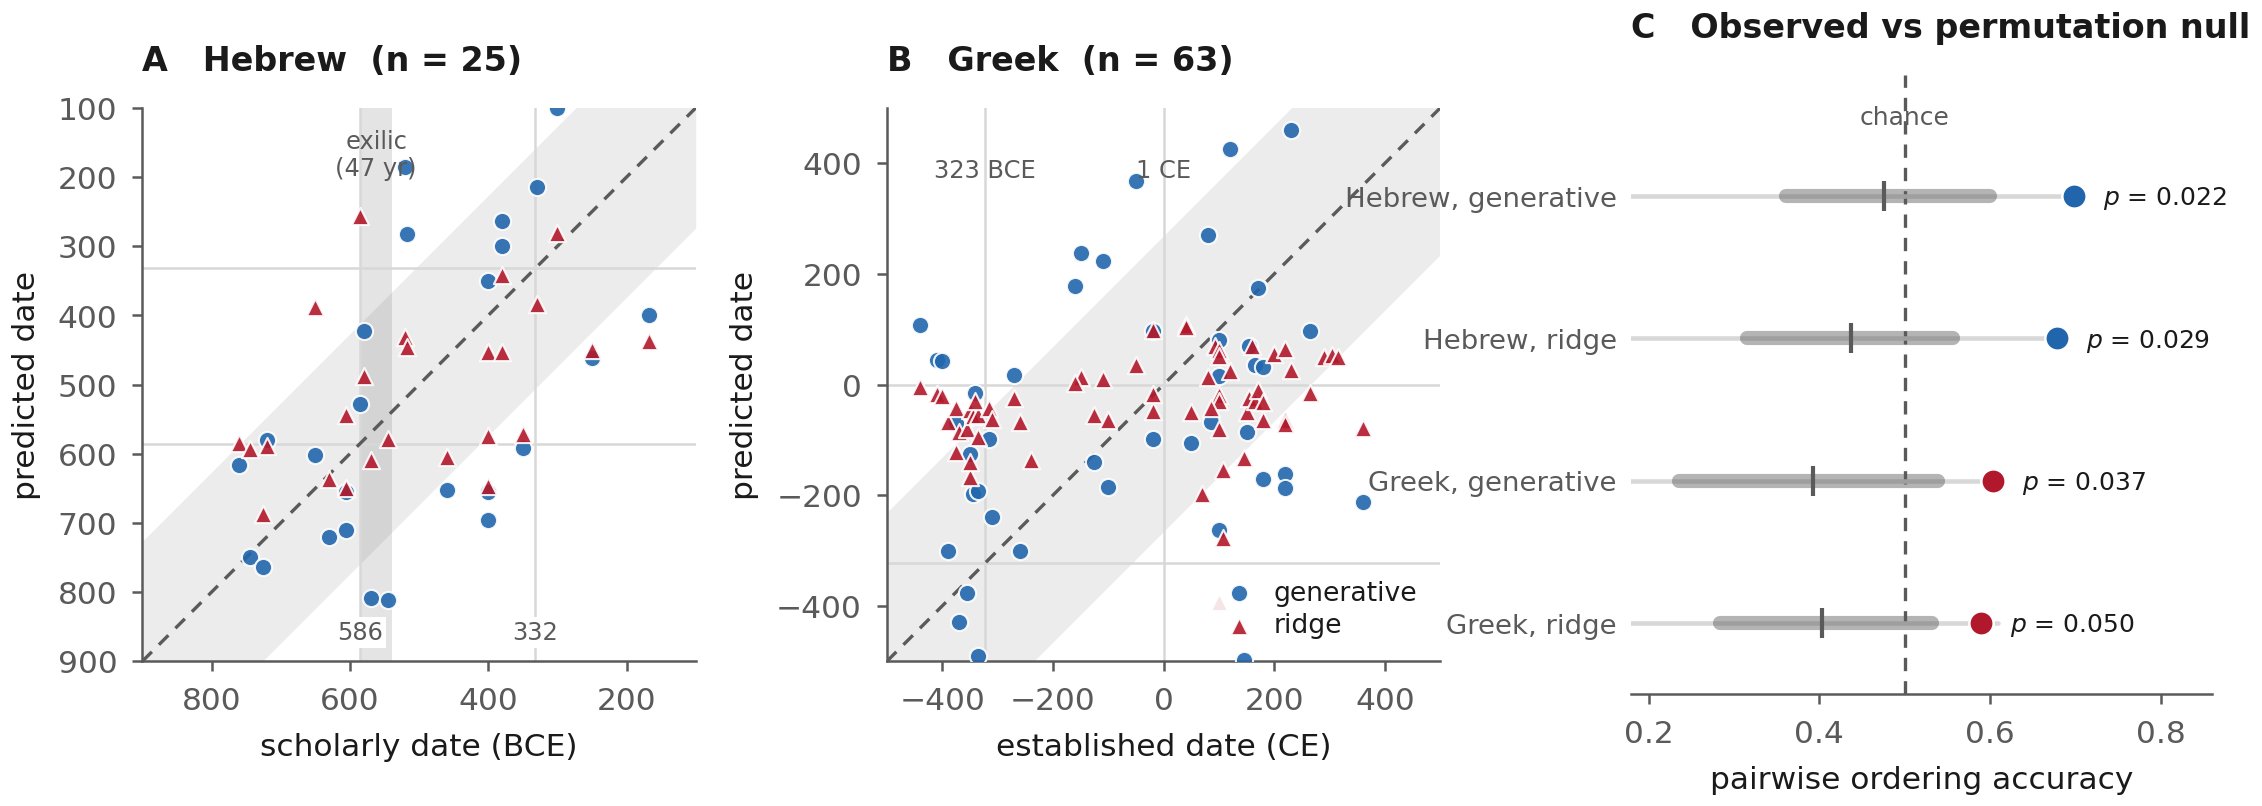
\includegraphics[width=\linewidth]{figures/fig1_ordering.png}
\caption{\textbf{The ordinal signal, under leakage-free cross-validation.}
\textbf{(A)}~Hebrew: scholarly date against leave-one-out predicted date for
all 25 dated units, both model families.  Time runs left to right on both
axes.  The dashed diagonal is perfect prediction and the shaded band is the
conformal 68\% interval.  The vertical strip marks the exilic window, 47~yr
wide against roughly 130~yr of irreducible error and therefore not
resolvable; vertical and horizontal rules mark the 586 and 332~BCE
boundaries.  \textbf{(B)}~Greek: the same analysis on 63 texts spanning
440~BCE--360~CE.  Scatter about the diagonal is proportionally larger
despite the larger corpus.  \textbf{(C)}~Pairwise ordering accuracy against
the permutation null.  Thin bars span the null 2.5--97.5 percentiles, thick
bars the interquartile range, the vertical tick the null mean; filled
markers are observed values.  The null is generated by shuffling the date
labels and re-running the entire pipeline, so it preserves the dependence
among pairs that a binomial test ignores.  All four observed values exceed
chance; none does so by a wide margin.}
\label{fig:ordering}
\end{figure}


\subsection*{What the signal does not support}

Absolute dating does not survive contact with an honest baseline.
Leave-one-out MAE is 156.2~yr for the generative family and 120.9~yr for
ridge.  Assigning every text the corpus mean date of 503~BCE gives 137.3~yr.
The generative family --- the one used for the point estimates reported in
earlier versions of this work --- is therefore \emph{worse} than a
constant, and ridge improves on a constant by 16~yr.  Any MAE figure in
this literature should be read against roughly 137~yr, not against zero.

Period assignment is correspondingly weak.  Four-way exact accuracy is
40.0\% (generative) and 48.0\% (ridge) against a 36\% majority-class
baseline; pre-exilic versus post-exilic classification reaches 72.0\% and
76.0\% against a 68\% baseline, significant in neither family
($p = 0.107$, $0.070$).  Across ten tests --- five metrics in two families,
strongly correlated --- nothing survives Benjamini-Hochberg correction at
$q = 0.05$, and four results survive at $q = 0.10$.  We report this
directly: no individual accuracy claim in this paper is robust to
multiplicity correction, and the ordinal result is defended on replication
across model families rather than on any single $p$-value.

The failure is structured rather than random.  The Exilic period is a
47-year window set against roughly 130~yr of irreducible error, and it is
simply not resolvable: of four exilic texts, the generative family places
none correctly and ridge one.  Hellenistic units collapse into Persian.
Pre-exilic is the only period the models recover reliably, and it is
recovered because it is wide and terminal, not because early Hebrew is
distinctive in some way the interior boundaries are not.

\subsection*{Calibration}

The parametric intervals used in earlier versions of this work achieve
52\% empirical coverage at a nominal 68\% (61\% under the residual
formulation; the manuscript previously reported 32\% for the original
specification).  The mechanism is visible in the multiverse analysis:
chance-correlated features receive large fitted coefficients and small
residual variances, and because the multivariate normal likelihood weights
each feature by $1/\sigma_j$, adding noise features \emph{narrows} the
credible interval.  Adding six and then twelve pure-noise features to a
clean specification shrinks the 68\% HDI for the P source from 329 to 285
to 246~yr while moving the MAP by less than 50~yr.  Interval width in this
framework is not a reliable index of evidence.

We therefore replace parametric intervals with conformal prediction
intervals calibrated on the leave-one-out residuals of the dated corpus.
These are distribution-free and carry guaranteed finite-sample marginal
coverage under exchangeability.  The resulting half-widths are $\pm233$~yr
(generative) and $\pm174$~yr (ridge) at 68\%.  These are the intervals
reported in Table~\ref{tab:targets}.  Exchangeability between the
calibration units and the targets is an assumption and not a guarantee:
the calibration units are whole books or coherent sections, whereas several
targets are cross-book composites.  Residual magnitude shows no detectable
dependence on text length ($\rho = -0.23$, $p = 0.27$), which supports the
use of a single conformal width.

\begin{table}[!ht]
\centering
\caption{\textbf{Decomposition of posterior precision for dated units.}
$\sigma_{\text{prior}}$ is the stated uncertainty on the scholarly date;
$\sigma_{\text{post}}$ is the posterior standard deviation returned when that
date is used as the prior mean.  The implied likelihood width is recovered as
$\sigma_L = (\sigma_{\text{post}}^{-2} - \sigma_{\text{prior}}^{-2})^{-1/2}$,
and the final column gives the share of posterior precision contributed by the
linguistic data.  The near-exact recoveries reported for Haggai,
Zechariah~1--8 and Daniel in earlier versions of this work correspond to data
shares below 6\%.  Median over all 25 dated units:
$\sigma_{\text{post}}/\sigma_{\text{prior}} = 0.851$, median
$|{\rm MAP} - d_u| = 10.4$~yr.}
\begin{tabular}{lrrrrr}
\hline
\textbf{Unit} & $\mathbf{d_u}$ & $\mathbf{\sigma_{\text{prior}}}$ & $\mathbf{\sigma_{\text{post}}}$ & $\mathbf{\sigma_L}$ & \textbf{data share} \\
 & (BCE) & (yr) & (yr) & (yr) & (\%) \\
\hline
Zechariah 1--8      & 518 & 10 & 9.8 & 53 & 3.4 \\
Haggai              & 520 & 10 & 9.9 & 58 & 2.8 \\
Daniel (Heb.)       & 167 & 10 & 9.7 & 41 & 5.5 \\
Amos                & 760 & 20 & 18.7 & 52 & 12.9 \\
Ezekiel             & 580 & 20 & 18.5 & 49 & 14.5 \\
Habakkuk            & 605 & 20 & 18.4 & 46 & 15.7 \\
Jeremiah oracle     & 605 & 30 & 25.5 & 49 & 27.6 \\
Chronicles          & 330 & 40 & 28.7 & 41 & 48.4 \\
Isaiah 56--66       & 400 & 100 & 45.0 & 50 & 79.8 \\
Ecclesiastes        & 250 & 120 & 40.7 & 43 & 88.5 \\
Joel                & 400 & 150 & 46.5 & 49 & 90.4 \\
Zechariah 9--14     & 350 & 150 & 39.4 & 41 & 93.1 \\
\hline
\end{tabular}
\label{tab:leakage}
\end{table}

\section*{Results: dating the undated units}
\label{sec:results}

The framework is applied to nineteen undated units: the three documentary
source composites and their sub-strata, the five books of the Pentateuch,
the Deuteronomistic prose stratum of Jeremiah, and two poems traditionally
argued to be archaic.  Models are fitted on all 25 dated units; no target
contributes to its own prediction, and all targets are dated under an
agnostic prior.  Results are given in Table~\ref{tab:targets} as conformal
date ranges rather than point estimates, for the reasons set out in
\nameref{sec:validation}.

\subsection*{The post-exilic result}

One substantive claim survives at full strength.  The posterior predictive
probability that a unit postdates 586~BCE is $\geq 0.92$ under both model
families for the P source, the D source and its Code and Frame strata, the
JE source, and Leviticus~P; the Holiness Code reaches 0.76 in the
generative family and 0.92 in ridge.  This is a statement about which side
of a single boundary the predictive mass falls on, and it is the kind of
claim the data can carry: it requires the estimator to be approximately
unbiased, not precise.

The finding is robust in three respects that matter.  It holds under both
model families, which disagree substantially about point estimates ---
median difference 59~yr, with agreement on the single most likely period
for only 9 of 19 units.  It holds under the genre correction developed
below, which if anything moves the sources \emph{later}.  And it does not
depend on the interval width, since a doubling of the conformal half-width
would still leave the great majority of predictive mass after 586~BCE for
every source composite.

\subsection*{What cannot be claimed}

No unit in Table~\ref{tab:targets} has a 68\% interval confined to a
single conventional period.  All nineteen span between two and four.  The
P source is placed at 264~BCE (68\%: 497--31~BCE) by the generative family
and 344~BCE (518--170~BCE) by ridge; these overlap comfortably, but they
straddle the Persian--Hellenistic boundary in both cases.  Earlier versions
of this work reported the P source at 361 and 404~BCE under two models and
described the result as Persian-period.  That characterisation is not
supportable.  What is supportable is that P is post-exilic and that its
predictive distribution is concentrated in the fourth and third centuries.

We note also that D~source and Deuteronomy are the same text and must not
be read as independent confirmations, and that the sub-strata of a source
are not independent of the composite that contains them.

\subsection*{The archaic poems}

The Song of the Sea (Exod~15) and the Song of Deborah (Judg~5) are the two
earliest of all nineteen targets in both model families, and the only
targets whose predictive mass sits predominantly before 586~BCE
($P_{\mathrm{post}} = 0.40$ and $0.48$ generative, $0.48$ and $0.48$
ridge).  Neither poem was used in training or in feature screening.

This is an out-of-sample check on an independently motivated hypothesis,
and the model passes it: the two texts most widely argued on comparative
Semitic and orthographic grounds to be the oldest Hebrew poetry are the two
the model places earliest, out of nineteen candidates, in both families.
We report it as corroboration of the ordinal signal rather than as a dating
of either poem, whose intervals (887--421 and 843--377~BCE, generative)
are far too wide to adjudicate the question they are usually asked to
settle.  In particular, the present analysis cannot distinguish a genuinely
early poem from a later archaizing composition; the resistant-model
diagnostic offered for that purpose in an earlier version of this work did
not function, returning zero flagged features across all 44 units, and has
been withdrawn.

\subsection*{Genre as a confound}

The dated corpus is 17/25 prophecy against 5 narrative, while the
Pentateuchal targets are predominantly narrative and legal.  A model
trained largely on prophecy and applied to narrative is exposed to exactly
the register confound this literature has long identified.

The confound is measurable in the leave-one-out residuals.  In the
generative family, narrative texts are dated $+112.4$~yr too late on
average while prophetic texts are dated $-25.1$~yr too early (Welch
$p = 0.016$).  In ridge the effect is absent ($-24.3$ versus $+31.3$~yr,
$p = 0.234$).  The disagreement between families is itself informative:
the bias is a property of the generative inversion, not of the features.

The direction matters for the substantive conclusion.  If narrative units
are systematically dated too late by roughly 112~yr in the generative
family, then the generative estimate for the P source should be corrected
\emph{earlier}, from 264~BCE to approximately 376~BCE --- which remains
firmly post-exilic, and which moves it toward the uncorrected ridge
estimate of 344~BCE rather than away from it.  The post-exilic conclusion
is therefore robust to the genre correction, and the two families converge
once the correction is applied.  We regard this as the strongest available
evidence that the post-exilic placement is not a register artifact, and we
note that it is available only because both families were fitted and
reported.

\begin{table}[!ht]
\centering
\caption{\textbf{Date ranges for undated units.}  Intervals are
conformal prediction intervals calibrated on leave-one-out residuals
from the dated corpus, and are therefore distribution-free with
guaranteed finite-sample marginal coverage; they replace the parametric
intervals used previously, which achieved 52\% empirical coverage at a
nominal 68\%.  Ranges are quoted earliest--latest in BCE.  $P_{\mathrm{post}}$
is the posterior predictive probability that the unit postdates 586~BCE,
reported as the \emph{lower} of the two model families at each row, so
the column is conservative with respect to model choice.
No unit has a 68\% interval confined to a single conventional period;
the ranges, not the period labels, are the result.  D source and
Deuteronomy are the same text and are not independent.
$^\dagger$Interval extends past 1~BCE; the later bound is quoted in CE.}
\begin{tabular}{lrrlrlr}
\hline
 & & \multicolumn{2}{c}{\textbf{Generative}} & \multicolumn{2}{c}{\textbf{Ridge}} & \\
\cline{3-4}\cline{5-6}
\textbf{Unit} & \textbf{Words} & \textbf{MAP} & \textbf{68\% range} & \textbf{MAP} & \textbf{68\% range} & \textbf{$P_{\mathrm{post}}$} \\
\hline
Song of the Sea     & 433 & 654 & 887--421 & 616 & 789--442 & 0.40 \\
Song of Deborah     & 462 & 610 & 843--377 & 614 & 787--440 & 0.48 \\
D Song              & 782 & 550 & 783--317 & 390 & 564--217 & 0.52 \\
Genesis JE          & 22{,}409 & 318 & 551--85 & 385 & 558--211 & 0.92 \\
Exodus JE           & 11{,}780 & 410 & 643--177 & 424 & 598--250 & 0.88 \\
Numbers JE          & 3{,}563 & 402 & 635--169 & 421 & 594--247 & 0.88 \\
JE source           & 37{,}752 & 356 & 589--123 & 400 & 574--226 & 0.92 \\
Holiness Code       & 5{,}958 & 464 & 697--231 & 344 & 518--171 & 0.76 \\
Leviticus P         & 10{,}496 & 256 & 489--23 & 315 & 489--142 & 0.96 \\
P source            & 54{,}435 & 264 & 497--31 & 344 & 518--170 & 0.92 \\
D Code              & 7{,}353 & 338 & 571--105 & 239 & 412--65 & 0.96 \\
D Frame             & 11{,}993 & 182 & 415--51~CE$^\dagger$ & 216 & 390--43 & 1.00 \\
D source            & 20{,}128 & 256 & 489--23 & 231 & 404--57 & 0.96 \\
Jeremiah Dtr        & 15{,}197 & 274 & 507--41 & 404 & 578--231 & 0.92 \\
Genesis             & 28{,}764 & 296 & 529--63 & 375 & 549--201 & 0.92 \\
Exodus              & 23{,}748 & 316 & 549--83 & 388 & 561--214 & 0.92 \\
Leviticus           & 17{,}099 & 342 & 575--109 & 326 & 500--153 & 0.92 \\
Numbers             & 23{,}188 & 274 & 507--41 & 375 & 549--202 & 0.92 \\
Deuteronomy         & 20{,}128 & 256 & 489--23 & 231 & 404--57 & 0.96 \\
\hline
\end{tabular}
\label{tab:targets}
\end{table}

\begin{figure}[!ht]
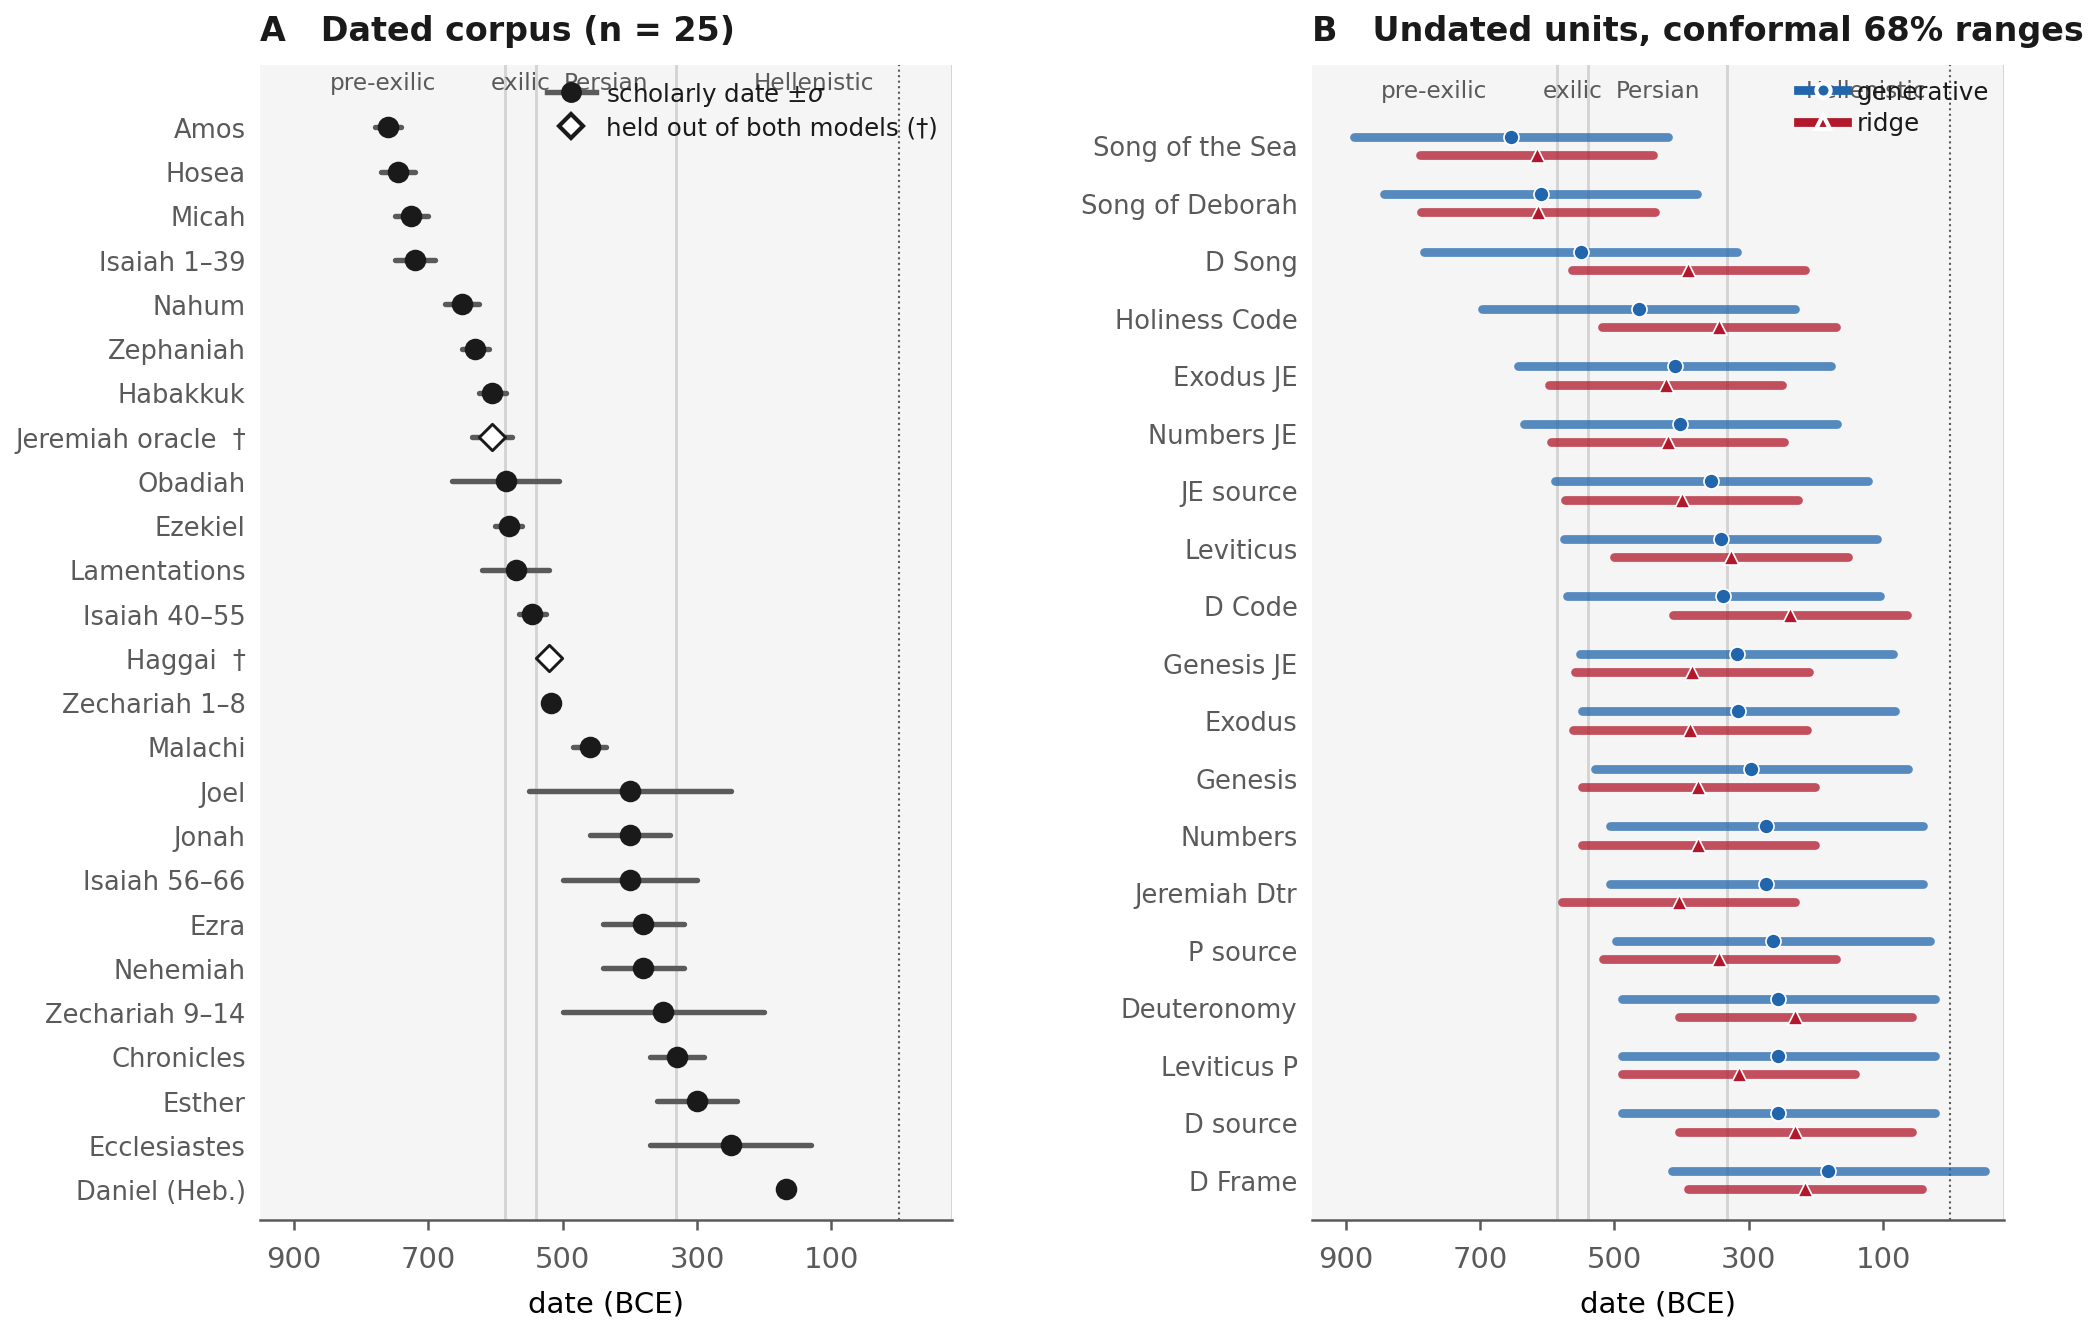
\includegraphics[width=\linewidth]{figures/fig2_timeline.png}
\caption{\textbf{Dated corpus and undated units on a common timeline.}
\textbf{(A)}~The 25 dated units with scholarly date and stated $\sigma$.
Widened sigmas on literary-critically dated texts (Joel, Zechariah~9--14,
Ecclesiastes, Isaiah~56--66, Obadiah) are visible as long bars.  Open
diamonds mark the two units held out of both models.  \textbf{(B)}~The 19
undated units with conformal 68\% ranges from both model families, ordered
by the generative point estimate.  No range is confined to a single period.
The Song of the Sea and the Song of Deborah are the earliest units under
both families and the only two whose mass sits predominantly before
586~BCE; neither was used in training.  Shaded bands are the conventional
periods, given for orientation only --- the ranges, not the band a range
happens to overlap, are the result.}
\label{fig:timeline}
\end{figure}


\section*{Discussion}
% -------------------------------------------------------

\subsection*{Limitations}

\textbf{Small training corpus.}  $N = 22$ dateable texts is small relative
to $J = 35$ features.  A stable $35 \times 35$ residual covariance
matrix requires at minimum $J + 1 = 36$ observations; with $N = 22$ the
sample covariance is rank-deficient, which is precisely why Tikhonov
regularization ($\lambda = 0.10$) is required.  As a rough power guide:
strict Benjamini-Hochberg FDR control~\cite{Benjamini1995} at $\alpha = 0.05$ with $J = 35$
features would require approximately $N \geq 100$ texts for adequate
power, which is unavailable for Biblical Hebrew; the permissive $p < 0.30$
threshold is the appropriate response to this constraint, not a relaxed
standard.  The sensitivity analysis (Fig.~\ref{fig:prior_sensitivity})
shows that MAP estimates are stable to within $\pm 30$~yr across the
plausible regularization range $\lambda \in [0.05, 0.30]$, but credible
intervals widen by 50--70~yr at the upper end of that range.  No texts
with secure independent dates suitable for training are withheld; $N = 22$
reflects the genuine constraint imposed by the historical record, not an
analytical choice.  The relationship between text length and posterior
uncertainty is shown in S10~Fig.

\textbf{Residual circularity.}  Critics have long identified an
``unexamined literary-linguistic circularity'' at the heart of the
traditional method~\cite{Young2003,Young2008,Rezetko2014}: diagnostic
features are identified on texts assumed to be early or late, then
applied to date other texts, recovering the assumptions embedded in the
training corpus.  Defenders call the objection ``valid but misplaced,''
invoking the philosopher Nelson Goodman's argument that such circularity
is ``a virtuous one''~\cite{Hendel2018}.  The appeal misreads Goodman.
His ``virtuous circle'' describes epistemological reflective equilibrium:
inference rules and particular inferences are revised in light of each
other until they cohere --- neither side is held fixed; both are
candidates for revision.  Linguistic dating does not work this way.  The
assumed dates of the anchor texts are not tentative hypotheses subject to
revision; they define what counts as early or late Hebrew.  Classical
Biblical Hebrew features are extracted from the Pentateuch and Former
Prophets, assumed to be early.  Those features then ``confirm'' that the
Pentateuch is early.  The assumed date is not tested against the
linguistic signal; it \emph{generates} the linguistic signal used to
confirm it.  That is a vicious circle in the traditional sense: the
conclusion is embedded in the premises.

The prior sensitivity analysis replaces this philosophical standoff with
a per-text empirical measurement.  Texts classified as data-driven
($|\Delta_{AB}| < 30$~yr) are genuinely constrained by the linguistic
signal: an agnostic and an informed prior converge, and the assumed
training dates contribute little.  For prior-dominated texts
($|\Delta_{AB}| > 80$~yr), the circle is self-reinforcing: shift the
assumed training dates and the posteriors shift substantially, which is
precisely what a vicious circle predicts.  The classification does not
eliminate circularity --- the corpus dates remain grounded in scholarly
tradition --- but it identifies, for each text, whether the circularity
is approximately benign or materially compromising.

The critique can be made quantitative.  We hold the linguistic feature
vectors for P, D, and JE fixed (reconstructed from MLE-MVN archaism
scores; see Methods) and vary only the Gaussian prior
$\mathcal{N}(\mu_0,\sigma_0^2)$ across six scenarios: an uninformative
flat (data-only) prior, the agnostic Mode-B prior
$\mathcal{N}(575,400^2)$, a tight scholarly prior
$\mathcal{N}(625,100^2)$ reflecting the Josianic--Persian consensus,
and two explicitly traditionalist assumptions, an early-monarchy prior
$\mathcal{N}(850,150^2)$ and a Mosaic-authorship prior
$\mathcal{N}(1200,100^2)$ centered on the conventional Exodus date
(Fig.~S14; S6~Table).  The feature likelihoods are identical across
all rows; only the prior changes.

Under the data-only (flat) prior, the MLE-MVN MAP dates are 357~BCE
(P), 294~BCE (D), and 434~BCE (JE) --- all within the Persian period.
Under the Mosaic prior $\mathcal{N}(1200,100^2)$ these shift to
444~BCE (P), 403~BCE (D), and 511~BCE (JE) --- still entirely within
the Persian period (539--332~BCE).  The prior cannot move any source
into pre-exilic territory because the linguistic signal is too
strongly inconsistent with such a date.  For P, which carries the
strongest data signal ($n = 53{,}645$~words), the total prior-induced
shift across the full range from flat to Mosaic is 87~yr, confirming
the data-driven classification from the prior sensitivity analysis.

A pre-exilic Torah date would require, on this account, either forcing
a prior so extreme that it overwhelms a directly contradictory data
signal, or including Torah texts in the training corpus so that
``Classical Biblical Hebrew'' features are extracted partly from
passages assumed to be early --- the traditional procedure, and
precisely the vicious circle identified above.  The present model uses
neither route: the training corpus excludes Torah and DH texts
entirely, and the prior is set before fitting.  The circularity is
thus not a philosophical abstraction but a measurable discrepancy
between prior assumptions and the linguistic record.

\textbf{Oral prehistory.}  The framework dates the written linguistic
surface.  Oral traditions preserved in written texts --- possible for
archaic poetry, legal formulae, or tribal lore --- are invisible to the
model; dates represent the written composition, not any hypothetical
prior oral form.

\textbf{Coarse genre correction.}  Genre is modeled at three levels
(prophetic, narrative, legal).  Sub-genre distinctions
(apodictic vs.\ casuistic law; etiological vs.\ court narrative) require
a larger corpus before they can be treated as distinct classes.

\textbf{Word n-gram limitations for short texts.}  Texts under
$\sim$1{,}000 words yield noisy POS-tag n-gram frequencies.  Short units
(Obadiah: 291~words; Haggai: 670~words) are flagged and results treated
as indicative.

\textbf{Legal prose genre gap.}  The training corpus covers prophetic,
poetic, narrative, and wisdom texts but contains no legal prose.  The
three Torah source composites include substantial legal sections ---
apodictic and casuistic law, cultic regulations, purity codes --- whose
register may differ from narrative prose for reasons unrelated to date.
Features with strong genre bias (genre ratio $\gamma_j > 1.5$; S1~Table)
are excluded from the model feature set.  The residual analysis reported
under \nameref{sec:results} quantifies what remains: in the generative
family narrative units are dated $+112$~yr too late relative to prophetic
units (Welch $p = 0.016$), an effect absent in ridge ($p = 0.234$).
However, genre confounds not captured by the three-level register
classification cannot be ruled out.  The results for D and P should be
read in light of this gap; the consistent post-exilic direction across
both models and across multiple feature exclusion schemes (S4~Table)
provides some assurance that the gap is not driving the headline finding,
but it remains a genuine limitation.

\textbf{Source-decomposition uncertainty.}  The documentary source
composites follow the standard critical partition of Baden~\cite{Baden2012}.
Any mis-assigned verses alter the feature vector and through it the MAP
date.  The robustness check in S4~Table suggests dates are stable to
$\sim$20~yr under moderate feature perturbations; however, a systematic
re-assignment of a major block --- for example, treating the Holiness Code
as a pre-Priestly stratum independent of P --- could shift MAP estimates
by a larger amount.  Scholars who adopt a different documentary partition
should re-extract feature vectors from their preferred source boundaries
before interpreting the model output.

\textbf{Training boundary and extrapolation.}  The \mvn{} corpus spans
760--167~BCE; the \hbvi{} training subset, which excludes Daniel, spans
760--330~BCE, so \hbvi{} dates near the late end are already mild
extrapolations.  Dates for texts composed before 760~BCE or
after 167~BCE carry no calibration constraint and should be interpreted
accordingly.  The \mvn{} date grid imposes hard boundaries at 900~BCE
and 100~CE; a composition outside this range would be pinned to the
nearest edge.

\textbf{Posterior overconfidence and calibration.}  The word-count
scaling factor $\mathrm{clip}(n/5000,1,5)$ sharpens posteriors for large
texts in a way that is not fully calibrated.  The LOO analysis
(Fig.~S13) shows that nominal 68\% credible intervals achieve only 32\%
actual coverage; a nominal 97.5\% CI is required to reach 68\% actual
coverage.  Any quoted credible interval should be read with this in mind;
for high-stakes applications the calibration-corrected interval is
preferable to the nominal one.

\subsection*{Scholarly context for late Torah dating}

The MAP dates returned for the documentary sources ---
P at $\sim$359~BCE, D at $\sim$294~BCE, and JE at $\sim$434~BCE under the
agnostic prior --- depart substantially from the mainstream critical
consensus, which conventionally places J and E in the 9th--8th
centuries~BCE, D in the 7th century (Josianic reform, $\sim$621~BCE), and
P in the late pre-exilic or early exilic
period~\cite{Wellhausen1885,Baden2012}.  The present framework does not
dispute that underlying oral traditions, archaic legal formulae, or early
poetic fragments may be considerably older; as noted in the Limitations
section above, the model dates the written linguistic surface of the final
composite texts, not any hypothetical prior oral stage.  Even within
mainstream critical scholarship, it is widely acknowledged that the
canonical forms of the sources passed through substantial post-exilic
editorial stages~\cite{CarrFormation2011,Romer2005}, so the question at
issue is not whether post-exilic editing occurred but how much of the
final written form it accounts for.

The results find independent support from several recent lines of
inquiry, perhaps the more striking for involving entirely different
methods.  Adler's comprehensive archaeological survey of the material
record finds no evidence for widespread observance of Torah regulations
--- dietary prohibitions, miqvaot, stone-vessel purity practice ---
before the mid-Hasmonean period (mid-2nd century~BCE)~\cite{Adler2022}.
If the Torah had functioned as a widely observed legal code since the
pre-exilic or early post-exilic period, the near-total absence of its
material correlates for several subsequent centuries would require
explanation; Adler concludes instead that the Torah achieved normative
authority only in the Hasmonean period, consistent with our model
returning Persian-period dates for the final written forms of P and D.
Epigraphic analysis of Achaemenid-era Aramaic sources similarly places
the crystallization of distinctively Jewish legal practice --- including
Passover regulations that the Priestly source legislates --- under
Persian imperial influence in the 5th--4th centuries~BCE~\cite{Barnea2026}.
On the other hand, independent study of the Moses tradition traces the
figure to a 4th-century~BCE literary construction drawing on Egyptian
folk-heroic conventions, locating even the narrative scaffolding of the
Pentateuch in the late Persian or early Hellenistic
period~\cite{Adair2025}.  An older body of historical-critical scholarship
has argued for Persian or Hellenistic final composition on
literary-historical grounds~\cite{Thompson1999,Lemche2008,Davies1992};
the empirical lines above are independent of that tradition and rest on
material and philological evidence rather than literary-critical
inference.

What the convergence suggests is something stronger than any single line
of evidence could provide on its own: the agreement cannot be an artifact
of shared assumptions, since the computational method makes no use of
historical, archaeological, or narrative-critical evidence in its
inference.  The present results would thus appear to constitute a fourth
independent line of confirmation --- from morphosyntactic and lexical
feature distributions, with no assumption about Torah composition date
built in --- agreeing with what archaeology, epigraphy, and comparative
mythology have separately indicated.

\subsection*{Extensibility}

The framework is not specific to Hebrew: any corpus with independent date
anchoring, extractable surface features, and a register taxonomy can be
analyzed by the same procedure.  Among the most promising near-term
applications are Qumran sectarian texts (1QS, CD, 1QM), which would allow
a quantitative test of the archaizing-register hypothesis; Akkadian
administrative archives, where Old Babylonian versus Neo-Babylonian feature
shifts in cuneiform corpora present a natural analogue; and Greek papyri
from Oxyrhynchus, which span the Ptolemaic through Byzantine periods in a
continuous documentary record.

The methodological cautions are equally portable.  Any application of
this framework to a new corpus should report the likelihood-only estimate
alongside the posterior, the share of posterior precision contributed by
the data, and a permutation null obtained by re-running the entire
pipeline on shuffled labels.  Each of these is inexpensive, and each
would have caught the failure documented here.

\subsection*{Relationship to authorship-attribution approaches}

The present framework is designed to complement rather than supersede
authorship-attribution methods such as the unsupervised document
decomposition of Koppel et al.~\cite{Koppel2011} and the Higher Criticism
discrepancy method of Faigenbaum-Golovin et al.~\cite{Faigenbaum2025}.
The latter excels at assigning disputed passages to known scribal schools
and at identifying the specific lemmas driving that assignment, grounding
computational results in categories already meaningful to philologists.
The present framework, on the other hand, is oriented toward
chronological ordering with calibrated uncertainty and toward quantifying
how much of a reported date is contributed by the evidence rather than the
prior --- questions the HC method was not designed to address.  Our
results suggest the two are complementary in a specific way: the HC
method's categorical assignments are robust where our calendar-year
estimates are not, while our ordinal statistics remain informative where
scribal-school membership is undefined.

How the two approaches might be combined is perhaps the most interesting
methodological question for future work.  A plausible joint analysis would
proceed in two stages: first, apply the HC method to determine the most
likely scribal milieu, which directly informs the register prior in
\hbvi{} --- a strong HC assignment to D/DtrH would motivate an SBH
register prior, while a P assignment would motivate Transitional or LBH;
then apply \hbvi{} with that informed prior to obtain a date posterior and
an ordinal position with calibrated uncertainty.  The relationship also
runs in reverse: a unit whose predictive mass lies overwhelmingly after
586~BCE constrains the plausible compositional settings for HC attribution
decisions, even when its calendar-year estimate is too diffuse to be
useful on its own.

% -------------------------------------------------------
\section*{Conclusion}

Whether the morphosyntax of Biblical Hebrew carries a usable diachronic
signal has been disputed for two decades, with one side treating linguistic
dating as an established instrument and the other arguing that its apparent
successes are circular.  The analysis reported here supports a position
available to neither camp as usually stated: the signal is real, the
circularity is real, and the two facts are compatible.

The signal is real in a specific and testable sense.  Under a design in
which no text contributes to its own prediction and significance is
established by permuting date labels through the entire pipeline, Hebrew
morphosyntactic features order text pairs chronologically at 69.8\% and
67.8\% accuracy against a permutation null near 45\% ($p = 0.022$,
$0.029$), and leave-one-out rank correlations reach $+0.58$ and $+0.49$ in
two independently specified model families.  These are not large effects,
but they are not chance, and they replicate --- across model families
within Hebrew, and across languages.

The circularity is real in an equally specific sense.  Holdout accuracies
of order 10--30~yr, reported in this literature and in earlier versions of
this work, arise when a held-out text is dated under a prior centred on the
scholarly date it is asked to recover.  For the most securely anchored
texts in the present corpus the linguistic evidence contributes under 6\%
of posterior precision, and the apparent recovery is a restatement of the
prior.  Corrected, the same design yields mean absolute errors near 100~yr
in Hebrew and near 120~yr in Greek.  We think it likely that this failure
mode is not confined to the present work, and we suggest that reported
holdout accuracies in this area be accompanied by the likelihood-only
estimate and by the fraction of posterior precision attributable to the
data.

What the corrected framework supports is narrower than what was previously
claimed and, we think, more useful.  It does not date texts: leave-one-out
error of 121--156~yr must be read against 137~yr for the trivial predictor
that assigns every text the corpus mean.  It does not assign texts to
historical periods with useful reliability, and it cannot resolve the
exilic period at all.  It does order texts, and it can determine on which
side of a well-separated boundary a text is likely to fall.  Applied to the
Pentateuchal sources under leakage-free conditions, that is enough to
establish that the Priestly, Deuteronomic and JE composites are post-exilic
with probability at least 0.92 under both model families and under a
correction for the genre imbalance of the training corpus --- and not
enough to place any of them within a particular post-exilic century.  For a
question that has been argued for a century and a half largely on
non-quantitative grounds, a bounded probabilistic answer to the coarse
question seems more valuable than an unbounded point estimate for the fine
one.

\section*{Supporting information}
% -------------------------------------------------------

\paragraph*{S1 Appendix.}
\label{S1_Appendix}
\textbf{Feature extraction pipeline and BHSA query code.}
Complete Python scripts for extracting all 35 morphosyntactic features and
56 word n-gram features from the BHSA/Text-Fabric database, including
feature definitions, normalization procedures, and chapter-range selectors
for sub-source extraction.

\paragraph*{S2 Appendix.}
\label{S2_Appendix}
\textbf{HB-VI model implementation.}
Complete \texttt{autograd}-based Python implementation of the hierarchical
Bayesian variational inference model, ADAM training loop, ELBO convergence
diagnostics, and date-posterior computation.

\paragraph*{S3 Appendix.}
\label{S3_Appendix}
\textbf{Prior sensitivity analysis: full results table.}
Complete Mode~A (scholarly prior) and Mode~B (agnostic prior) MAP dates and 68\% credible intervals
for all 15 analyzed texts (10 sub-sources plus the three comparison texts
Habakkuk, Haggai, and Daniel, plus the documentary composites D\_source
and JE\_source), with $\Delta_{AB}$ shift values and classification.

\paragraph*{S4 Appendix.}
\label{S4_Appendix}
\textbf{Ancient Greek corpus manifest.}
Complete list of 63 Ancient Greek training texts with author, work,
date (CE), register class assignment, and word count.  Texts are drawn
from the Perseus Digital Library~\cite{Perseus} and Thesaurus Linguae
Graecae~\cite{TLG}.

\paragraph*{S1 Fig.}
\label{S1_Fig}
\textbf{Archaism heatmap.}
Heat map of archaism index (full-model MAP minus resistant-model MAP)
across all analyzed textual units, grouped by register class (SBH,
Transitional, LBH) and text type (prophetic, narrative, legal).
Positive values (warm colors) indicate archaizing; negative values
(cool colors) indicate transmission-with-updating.

\paragraph*{S2 Fig.}
\label{S2_Fig}
\textbf{Archaism index versus Kings--Chronicles comparison.}
Archaism indices for texts with Kings--Chronicles parallel passages
(Isa~36--39 // 2~Kgs~18--20; Jer~52 // 2~Kgs~24--25; Ps~18 // 2~Sam~22).
Tests whether parallel transmission introduces systematic archaism bias.

\paragraph*{S3 Fig.}
\label{S3_Fig}
\textbf{PCA stylometric projection.}
Principal component analysis of all 35 morphosyntactic features across
the 22 training texts plus analyzed sub-sources.  Confirms that the
three register classes (SBH, Transitional, LBH) are linearly separable
in feature space, consistent with the regression model assumption.

\paragraph*{S4 Fig.}
\label{S4_Fig}
\textbf{Pentateuchal sub-source posteriors.}
Full posterior distributions for D\_source, P\_source, and JE\_source
under both the scholarly prior (Mode~A) and agnostic prior (Mode~B),
shown alongside the individual sub-unit posteriors (D\_Code, D\_Frame,
Lev\_Holiness, Lev\_Priestly, Gen/Exo/Num\_JE).

\paragraph*{S5 Fig.}
\label{S5_Fig}
\textbf{Word n-gram agreement plot.}
Agreement between word n-gram model MAP dates and MLE-MVN MAP dates
across all training texts and analyzed sub-sources, demonstrating
independent feature-type convergence for texts without archaizing signal.

\paragraph*{S6 Fig.}
\label{S6_Fig}
\textbf{Feature loadings (OLS slopes) for all 35 morphosyntactic features.}
Horizontal bar chart of $\hat{\beta}_j$ (OLS slope of feature rate against
date in BCE) with 95\% confidence intervals.  Features are sorted within
each tier by slope magnitude.  Blue = Tier~1 (lexical), green = Tier~2
(morphological), red = Tier~3 (resistant, marked [R]).  Negative slopes
indicate features that decline with date (more frequent in older texts);
positive slopes indicate features that rise with date (more frequent in
later texts).

\paragraph*{S7 Fig.}
\label{S7_Fig}
\textbf{Raw residual feature correlations (pre-regularisation).}
Pearson correlations among OLS residuals across the 22 training texts,
computed before Tikhonov regularisation ($\lambda = 0.10$).
Regularisation shrinks these entries toward zero to ensure invertibility
of the $35 \times 35$ covariance matrix ($N = 22 < J = 35$ makes the
raw matrix rank-deficient).  Within-tier correlations---particularly
negative coupling between complementary forms
(\textit{wayyiqtol}/\textit{qatal}, \textit{asher}/\textit{she-})---confirm
that features co-vary beyond the linear time trend, motivating the full
MVN likelihood over an independent-feature approximation.

\paragraph*{S8 Fig.}
\label{S8_Fig}
\textbf{MLE-MVN calibration: training-set MAP vs.\ scholarly date.}
Each of the 22 training texts is plotted at its scholarly date (x-axis)
versus the model MAP date (y-axis), with 68\% HDCI error bars.  Colors
indicate register class (blue = SBH, green = Transitional, red = LBH).
The dashed diagonal is perfect calibration.  The extremely narrow CIs
for within-group texts (median 3--4~yr) indicate the model is
overconfident in-sample.  This overconfidence is quantified under
\nameref{sec:validation} and is the reason the intervals reported in
Table~\ref{tab:targets} are conformal rather than parametric.

\paragraph*{S9 Fig.}
\label{S9_Fig}
\textbf{HB-VI ELBO convergence curve.}
Evidence lower bound (ELBO) as a function of ADAM iteration (learning
rate~= 0.02, 3{,}000 iterations).  The dashed vertical line marks the
80\% point beyond which improvement falls below 0.01\% per 100 iterations.
The inset shows the final 500 iterations; near-flat behaviour confirms
convergence was achieved well before 3{,}000 iterations.

\paragraph*{S10 Fig.}
\label{S10_Fig}
\textbf{68\% HDCI width vs.\ text length (MLE-MVN, training texts).}
Posterior uncertainty (68\% HDCI width in years) plotted against word
count on a log scale for all non-holdout training texts.  Shorter texts
(Nahum: 618~words; Haggai: 670~words) have wider posteriors, motivating
the caveat that results for texts under $\sim$1{,}000 words are indicative
rather than definitive.

\paragraph*{S12 Fig.}
\label{S12_Fig}
\textbf{Training corpus: texts, scholarly dates, and HB-VI MAP estimates.}
The 25 dated units (23 training, 2 held out of both models: the Jeremiah
oracular stratum and Haggai) plotted on
the BCE timeline.  Open markers show scholarly consensus dates $\pm\sigma$; filled
diamonds show HB-VI MAP estimates $\pm$ 68\% HDCI.  Color indicates register zone:
blue = SBH ($\sim$760--590~BCE), green = Transitional ($\sim$590--460~BCE),
red = LBH ($\sim$460--167~BCE).  The holdouts were excluded from training and used
solely for LOO cross-validation.

\paragraph*{S13 Fig.}
\label{S13_Fig}
\textbf{Leave-one-out (LOO) calibration analysis for the MLE-MVN model.}
(A) LOO-predicted MAP dates versus true (anchored) dates for all 22 training texts,
with 68\% credible-interval whiskers.  Error bars reflect the model's nominal 68\% CI;
the ±100~yr grey band shows the region of acceptable recovery.
(B) Calibration curve plotting nominal credible-interval level against the fraction of
LOO tests in which the true date falls inside that interval.  The model is systematically
overconfident: the nominal 68\% CI achieves only 32\% actual coverage, and a nominal
97.5\% CI is needed to recover 68\% actual coverage.  The inset box shows the
consequence for the Priestly source (P): its MAP date is 359~BCE (Persian--Hellenistic),
and even after expanding to the calibration-corrected 68\% interval ($\equiv$ nominal
97.5\%), the corrected interval is 285--435~BCE --- entirely post-exilic.
The largest LOO errors occur for Ezra (predicted $\sim$156~BCE, true 400~BCE),
Daniel (predicted $\sim$502~BCE, true 167~BCE), Ezekiel (predicted $\sim$382~BCE, true
570~BCE), and Ecclesiastes (predicted $\sim$539~BCE, true 330~BCE); all four are texts
with contested or debated traditional dates in the scholarship.

\paragraph*{S14 Fig.}
\label{S14_Fig}
\textbf{Circularity demonstration: prior sensitivity of Torah source dates.}
Normalised MLE-MVN posterior curves for (A) the Priestly source
($n=53{,}645$~words; data-driven) and (B) the Deuteronomist source
($n=20{,}128$~words; prior-dominated) under six prior assumptions: a
data-only flat prior (grey dotted), the agnostic prior
$\mathcal{N}(575,400^2)$ (blue solid), a tight scholarly prior
$\mathcal{N}(625,100^2)$ (orange dashed), an early-monarchy prior
$\mathcal{N}(850,150^2)$ (red dash-dot), a united-monarchy prior
$\mathcal{N}(1000,150^2)$ (purple long-dash), and a Mosaic-authorship
prior $\mathcal{N}(1200,100^2)$ (dark green dash-dot-dot).  The green
band marks the Persian period (539--332~BCE); the vertical dashed red
line marks the Babylonian destruction (586~BCE).  Feature likelihoods
are identical across all curves; only the prior assumption differs.
Even under the Mosaic prior, MAP dates are 444~BCE (P) and 403~BCE (D),
both within the Persian period.

\paragraph*{S6 Table.}
\label{S6_Table}
\textbf{Prior-sweep MAP dates for the three Torah source composites.}
MLE-MVN MAP dates (BCE) for P, D, and JE under six prior scenarios,
from a data-only flat prior to a Mosaic-authorship prior
$\mathcal{N}(1200,100^2)$.  Feature vectors are identical across all
rows; only the prior changes.  None of the six scenarios recovers a
pre-exilic MAP date for any source.

\paragraph*{S1 Table.}
\label{S1_Table}
\textbf{Full feature set.}
All 35 selected morphosyntactic features with Spearman $\rho$,
$p$-value, LOO retention fraction, genre ratio $\gamma_j$, and tier
assignment.

\paragraph*{S2 Table.}
\label{S2_Table}
\textbf{Word n-gram feature set.}
All 56 selected Type~A and Type~B n-gram features with Spearman $\rho$
and LOO retention fraction.

\paragraph*{S3 Table.}
\label{S3_Table}
\textbf{Top dating-driving features for the three Documentary Hypothesis source composites.}
For each source the three features most strongly indicating late composition and the three most
strongly indicating early composition are listed with their normalized archaism scores and a
note on potential genre confound.  Scores follow Eq.~\ref{eq:lbh_score}: 0 = CBH-like, 1
= LBH-like, $<0$ = more archaic than the CBH anchor, $>1$ = more LBH-like than the LBH
anchor.  This table is provided to allow readers to evaluate the model's inferences directly,
without relying on the fitted model weights.

\paragraph*{S4 Table.}
\label{S4_Table}
\textbf{Robustness check: MAP dates under progressive feature exclusion.}
The MLE-MVN model is refit after removing the two genre-flagged features identified in
S3~Table (\textit{asher} frequency for D; wayyiqtol fraction for JE) and after removing
all features with normalized archaism scores exceeding $|s|>2.5$ for any source.  Feature
vectors for D, P, and JE are reconstructed from normalized archaism scores (see Methods);
absolute dates carry a minor approximation error from this reconstruction, so the shift
columns ($\Delta$) are the primary quantities of interest.  All sources remain in the
Persian-to-Hellenistic period under all exclusion schemes.

\paragraph*{S5 Table.}
\label{S5_Table}
\textbf{Corpus word counts for training texts and out-of-sample sources.}
All word counts are morphological words (BHSA) excluding coordinating conjunctions.
The 19 training texts span 760--330~BCE and cover prophetic, poetic, narrative, and
wisdom registers; three additional texts (Habakkuk, Haggai, Daniel) serve as
cross-validation holdouts for the HB-VI model.  Documentary Hypothesis source composites
and sub-source divisions are excluded from both training and validation; their dates are
derived solely from the model posterior.

% -------------------------------------------------------
\section*{Data availability}
% -------------------------------------------------------

All feature extraction scripts, Bayesian dating models, prior sensitivity
code, and corpus manifests are publicly available at
\url{https://github.com/adairaar/diachronic-hebrew}.  The underlying Hebrew text corpus is the Biblia
Hebraica Stuttgartensia Amstelodamensis (\bhsa{}), version 2021,
available at \url{https://github.com/ETCBC/bhsa} under a Creative Commons
Attribution 4.0 license~\cite{BHSA2021}.  The Ancient Greek corpus is
drawn from the Perseus Digital Library (\url{http://www.perseus.tufts.edu})
and the Thesaurus Linguae Graecae (\url{http://stephanus.tlg.uci.edu}),
both publicly accessible.  No proprietary data were used.

% -------------------------------------------------------
\section*{Author contributions}
% -------------------------------------------------------

A.A. conceived and designed the study, developed and implemented all
computational methods, performed all analyses, interpreted the results,
and wrote the manuscript.

% -------------------------------------------------------
\section*{Competing interests}
% -------------------------------------------------------

The author declares no competing interests.

% -------------------------------------------------------
\section*{Funding}
% -------------------------------------------------------

The author received no specific funding for this work.

% -------------------------------------------------------
\section*{Ethics statement}
% -------------------------------------------------------

This study does not involve human participants, vertebrate animals,
or any data requiring ethical oversight.  All textual data analyzed are
publicly available historical corpora.  No ethical approval was required.
This study was not pre-registered; it is a methods paper reporting
retrospective analysis of existing corpora.

% -------------------------------------------------------
\section*{Acknowledgments}
% -------------------------------------------------------

The author thanks the ETCBC team for maintaining the Biblia Hebraica
Stuttgartensia Amstelodamensis (\bhsa{}) database and making it freely
available.

\nolinenumbers

% -------------------------------------------------------
\clearpage
\bibliography{references}
% -------------------------------------------------------

\clearpage
% -------------------------------------------------------
% Figures
% -------------------------------------------------------


\begin{figure}[!h]
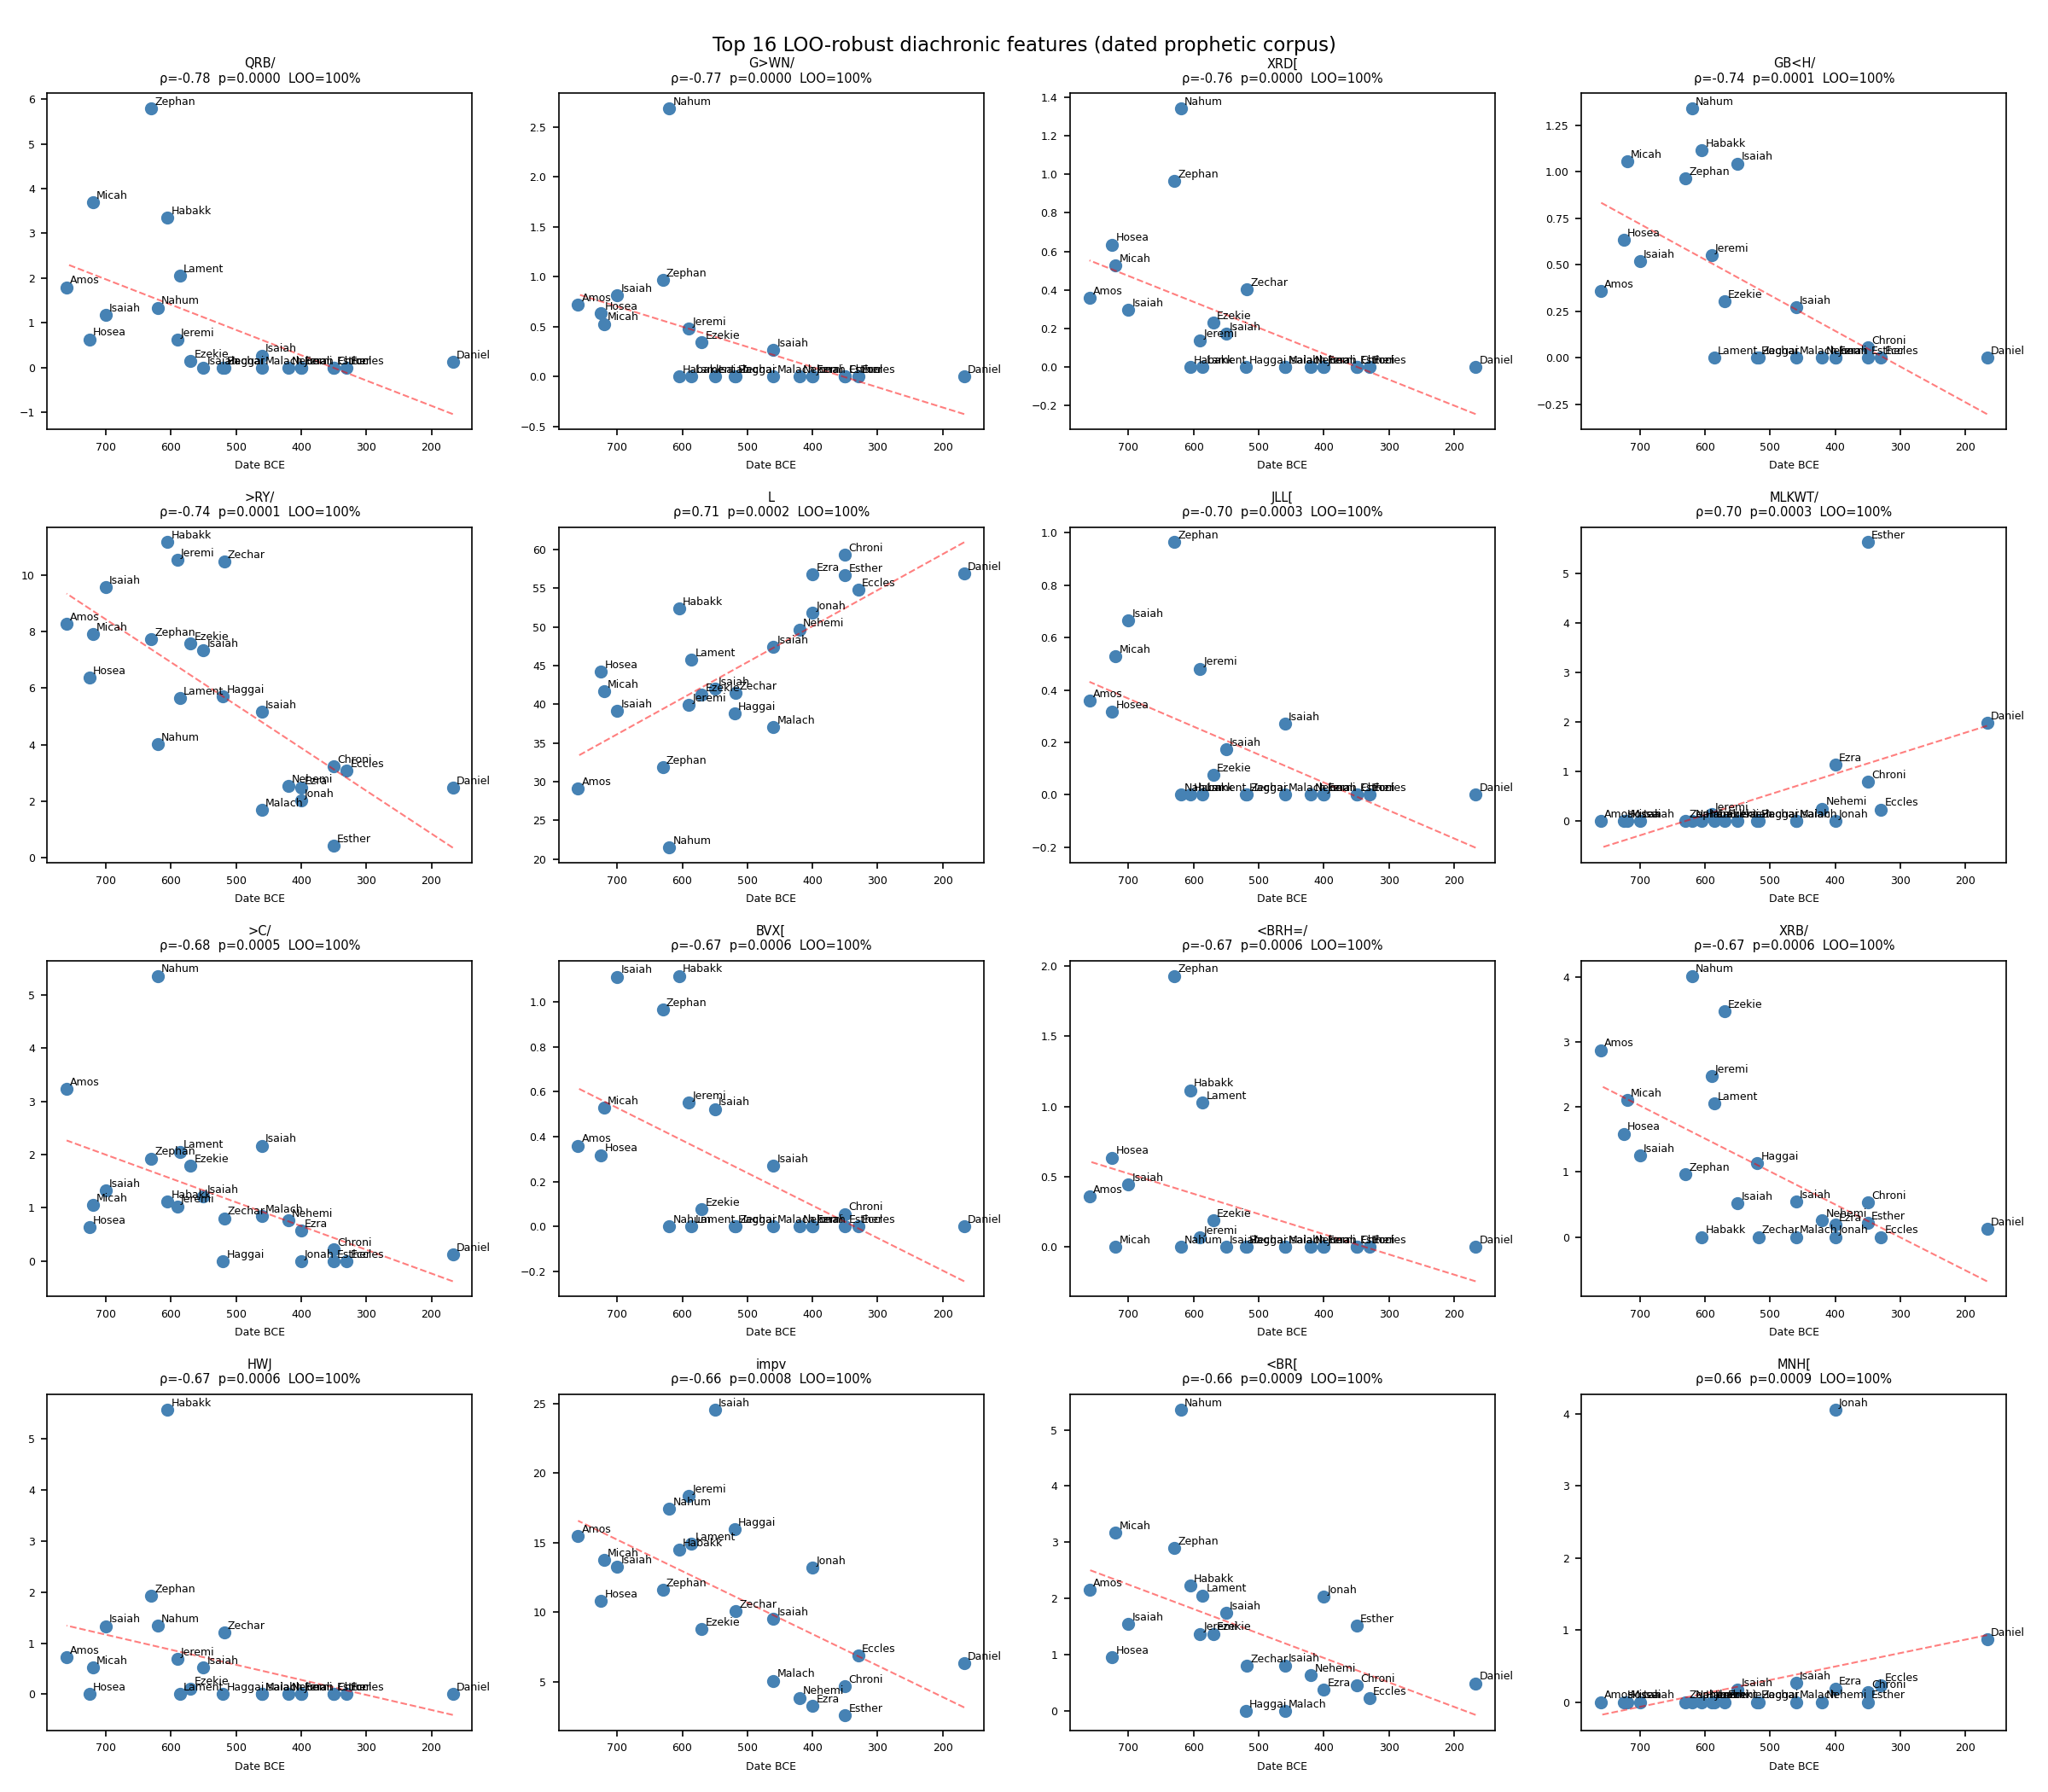
\includegraphics[width=\linewidth]{figures/fig2_feature_correlations.png}
\caption{\textbf{Top 16 LOO-robust diachronic features from the full
lexeme and morphological scan of the dated prophetic corpus.}
Each panel plots the per-1,000-word rate of one feature ($y$-axis) against
scholarly date BCE ($x$-axis; older texts at left) across all 22 training
units, with OLS trend line.  Spearman $\rho$, raw $p$-value, and
leave-one-out robustness fraction (LOO; proportion of LOO resamplings
returning the same sign and significance) appear above each panel; all
16 features achieve LOO~=~100\%.  Features marked SBH~$\downarrow$ are
characteristic of pre-exilic Classical Biblical Hebrew and decline toward
the post-exilic period; LBH~$\uparrow$ features show the reverse pattern.
The term \textit{malkut} (`kingdom'; a hallmark Late Biblical Hebrew noun)
and the rate of the preposition \textit{lamed} are the two LBH~$\uparrow$
markers in this set; the remaining 14 features are SBH markers that
decrease monotonically with date.  The feature labeled BVX is an
unidentified rare prophetic root in the BHSA lexicon.}
\label{fig:feature_correlations}
\end{figure}






\begin{figure}[!h]
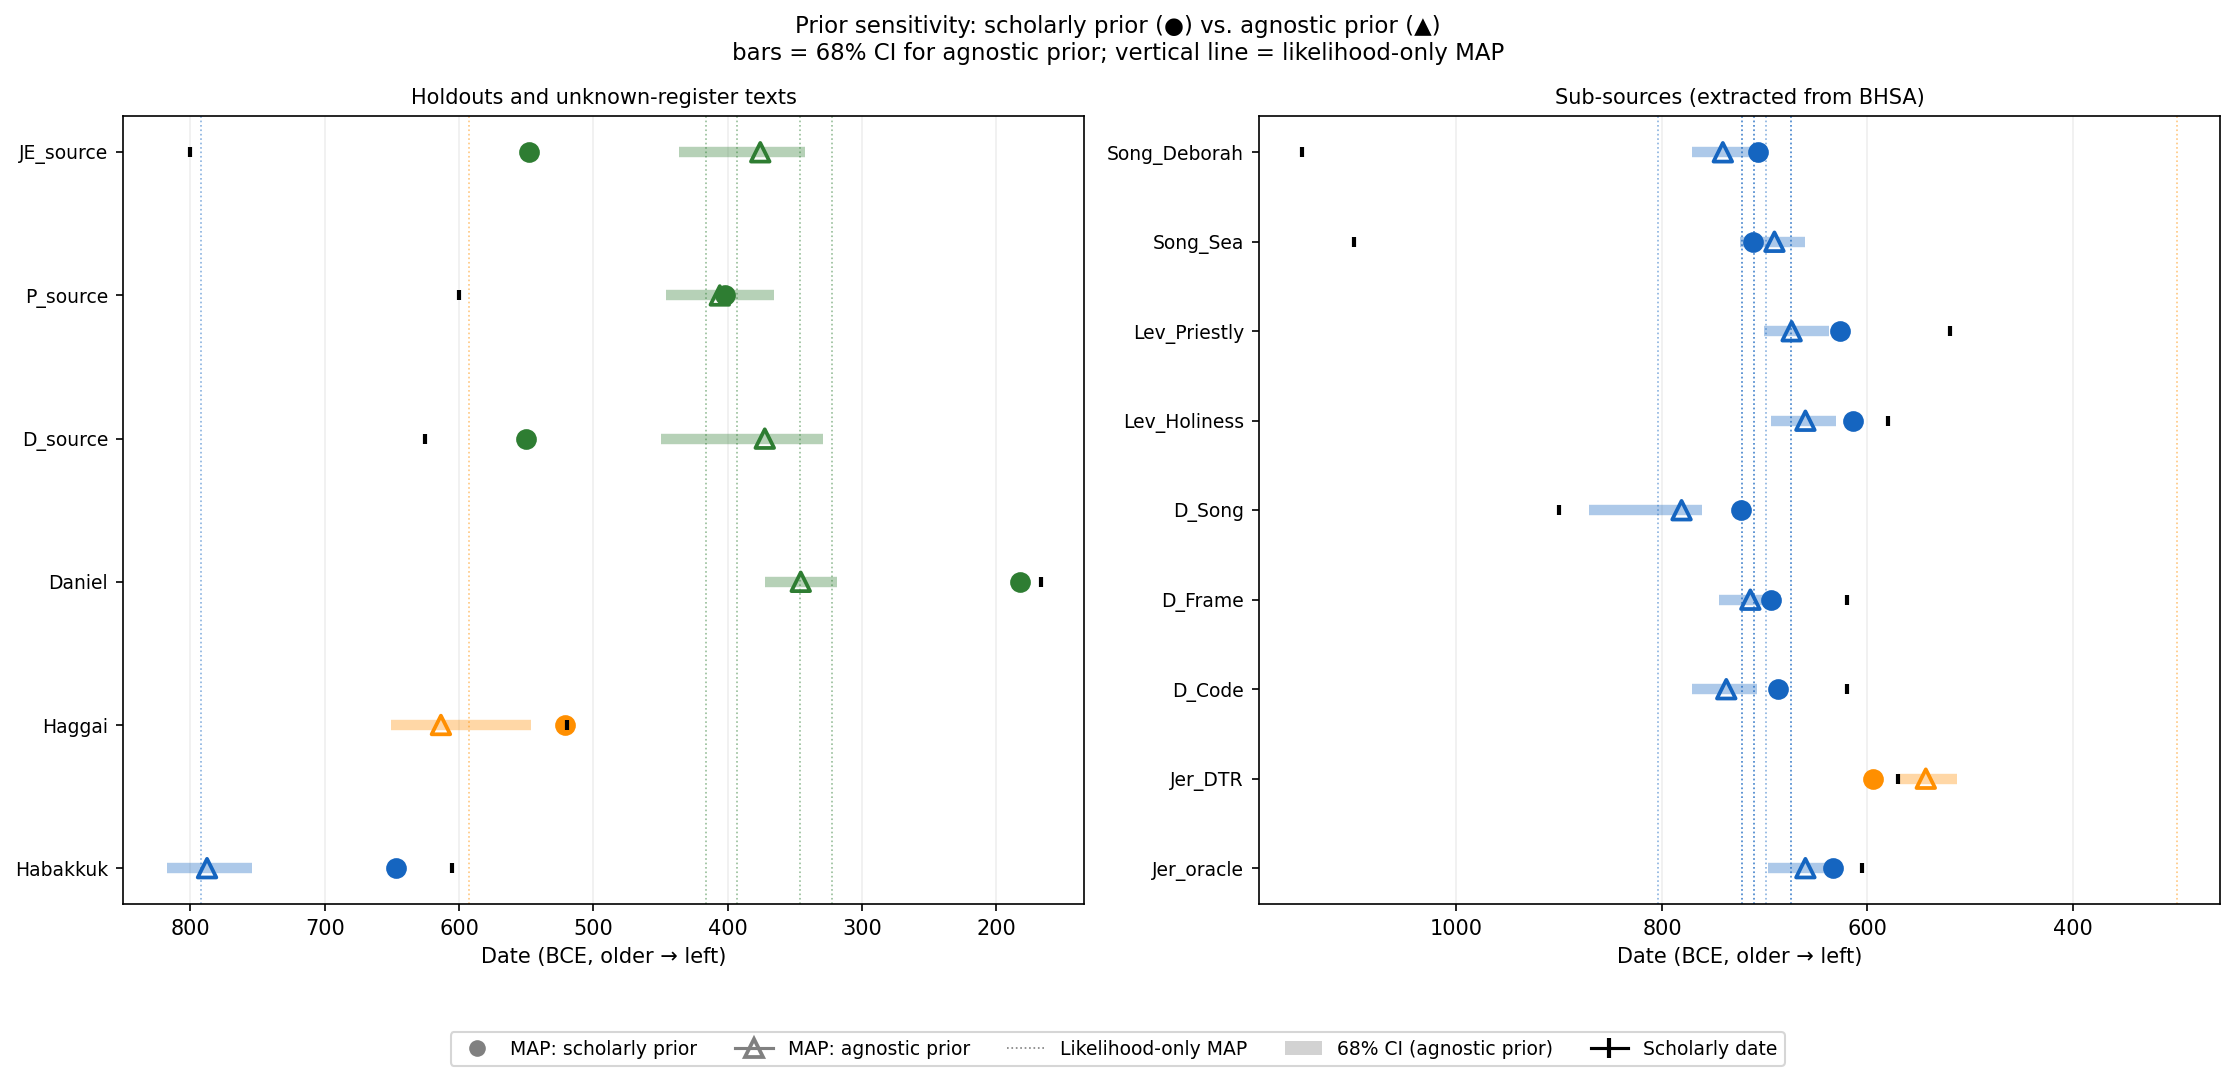
\includegraphics[width=\linewidth]{figures/fig8_prior_sensitivity.png}
\caption{\textbf{Prior sensitivity analysis: Mode~A versus Mode~B MAP
dates for all sub-sources.}
Mode~A (scholarly prior, circles) and Mode~B (agnostic prior, triangles)
MAP dates are connected for each text.  Line length represents the
$\Delta_{AB}$ shift; texts are colored by classification:
green~=~data-driven ($|\Delta_{AB}|{<}30$~yr),
orange~=~mildly prior-influenced (30--80~yr),
red~=~prior-dominated ($>80$~yr).
The four data-driven texts (Song\_Sea, P\_source, D\_Frame, Jer\_oracle)
are annotated.}
\label{fig:prior_sensitivity}
\end{figure}

\begin{figure}[!h]
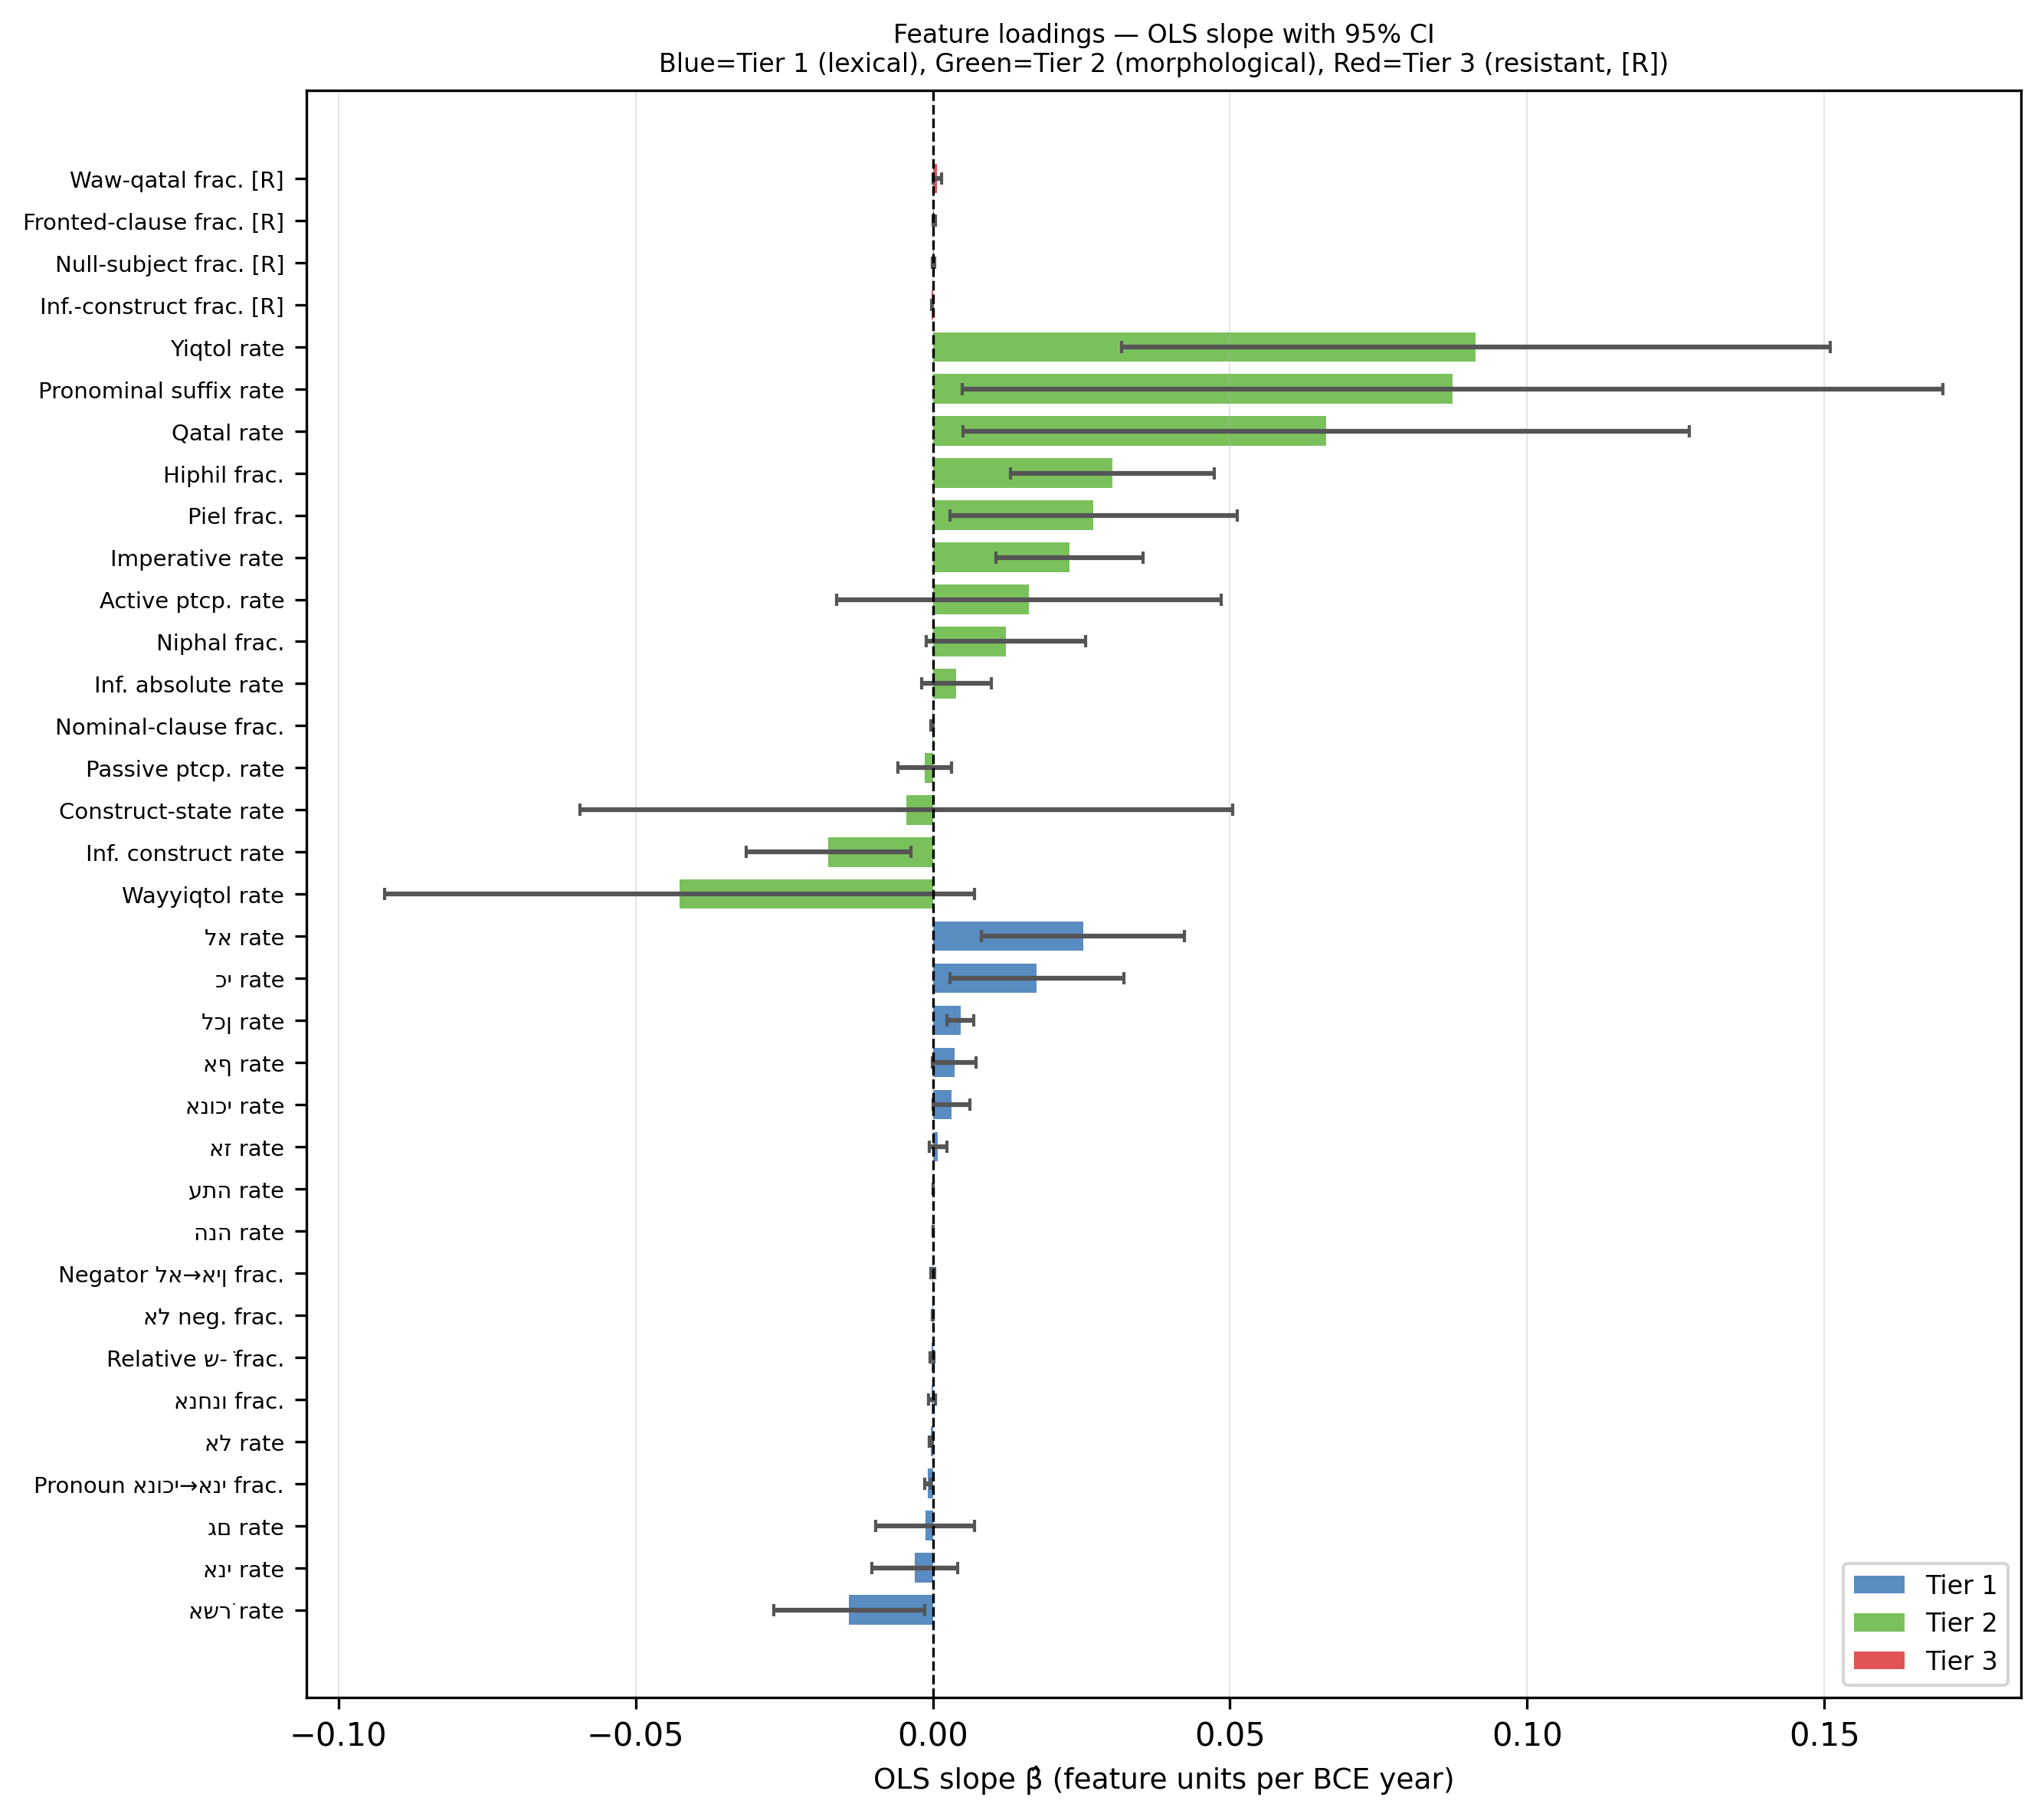
\includegraphics[width=\linewidth]{figures/fig_s6_feature_loadings.png}
\caption{\textbf{S6 Fig.\ Feature loadings (OLS slopes) for all 35 morphosyntactic features.}
$\hat{\beta}_j$ (OLS slope against date BCE) with 95\% CI.
Blue = Tier~1 (lexical), green = Tier~2 (morphological), red = Tier~3
(resistant, [R]).  Negative slopes = feature declines with date;
positive = rises with date.}
\label{fig:s6_loadings}
\end{figure}

\begin{figure}[!h]
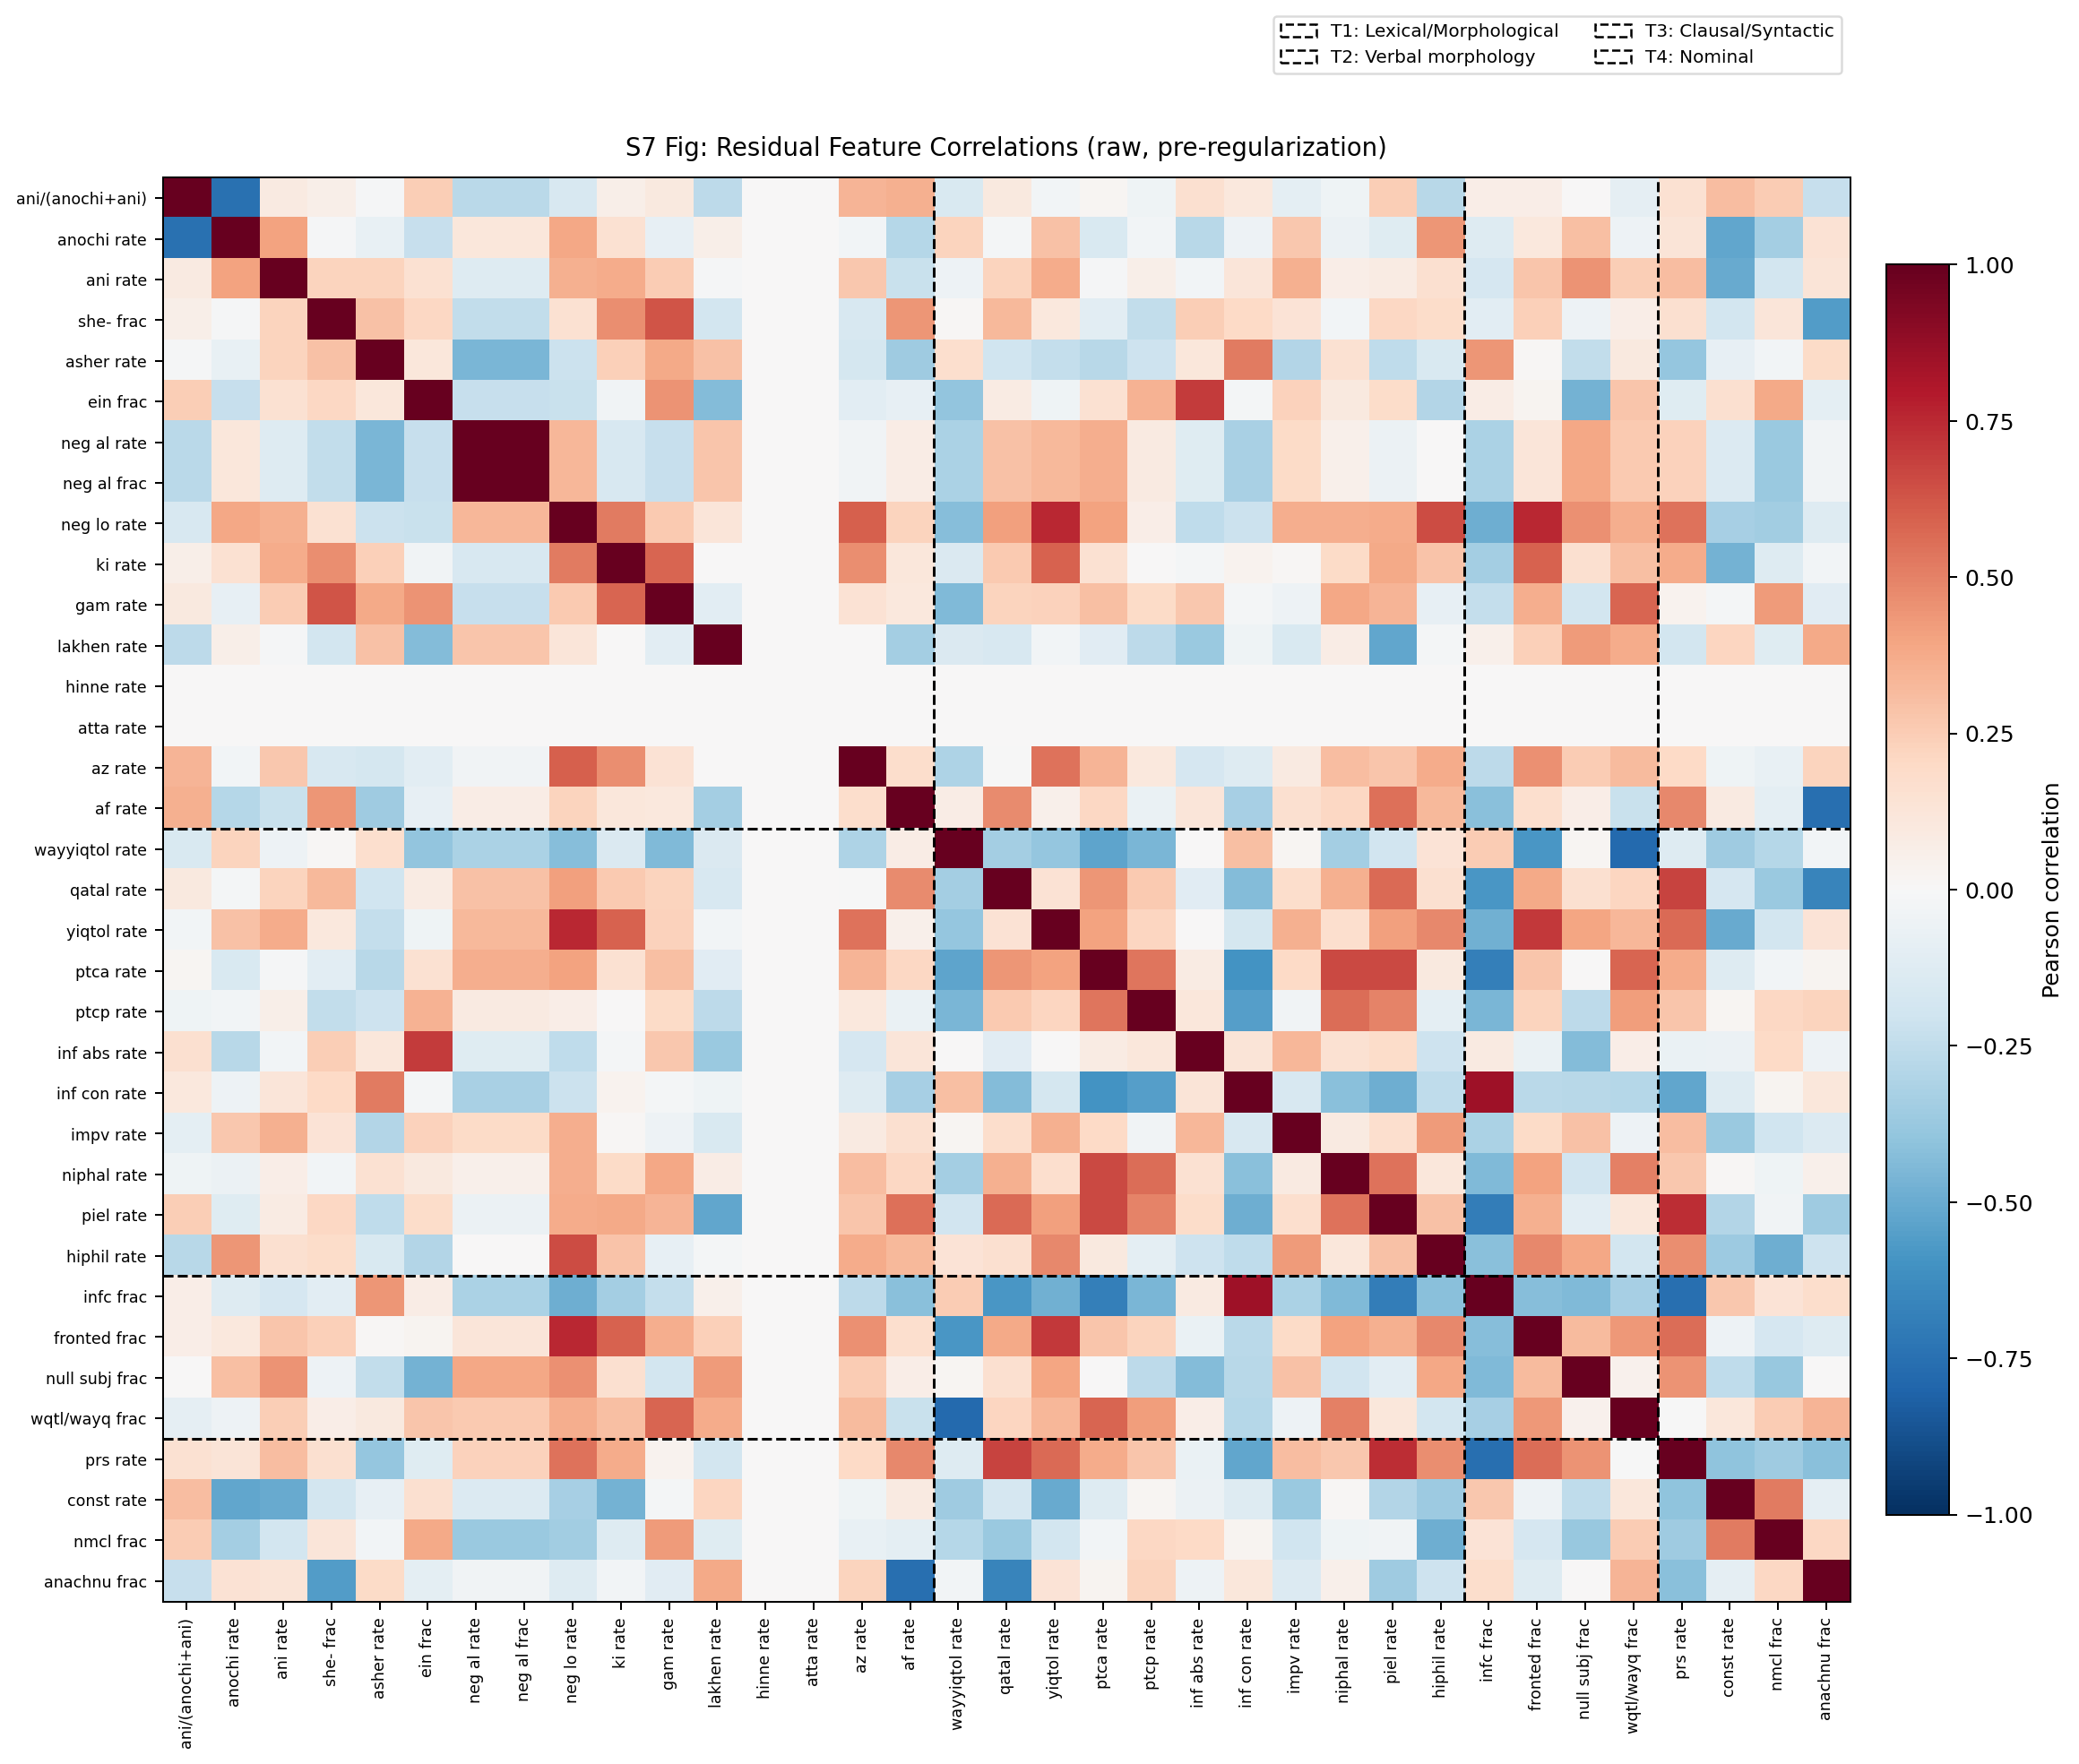
\includegraphics[width=\linewidth]{figures/fig_s7_covariance_heatmap.png}
\caption{\textbf{S7 Fig.\ Raw residual feature correlations (pre-regularisation).}
Pearson correlations among OLS residuals across the 22 training texts, computed
\emph{before} Tikhonov regularisation ($\lambda = 0.10$).  Regularisation
shrinks these off-diagonal entries toward zero to ensure the $35 \times 35$
covariance matrix $\Smat$ is invertible (the raw matrix is rank-deficient
because $N = 22 < J = 35$).  Tier boundaries are marked by dashed lines.
Within-tier correlations---particularly the negative coupling between
complementary forms (e.g., \textit{wayyiqtol}/\textit{qatal},
\textit{asher}/\textit{she-})---confirm that features co-vary beyond the
linear time trend, motivating the full MVN likelihood over an
independent-feature approximation.}
\label{fig:s7_covariance}
\end{figure}


\begin{figure}[!h]
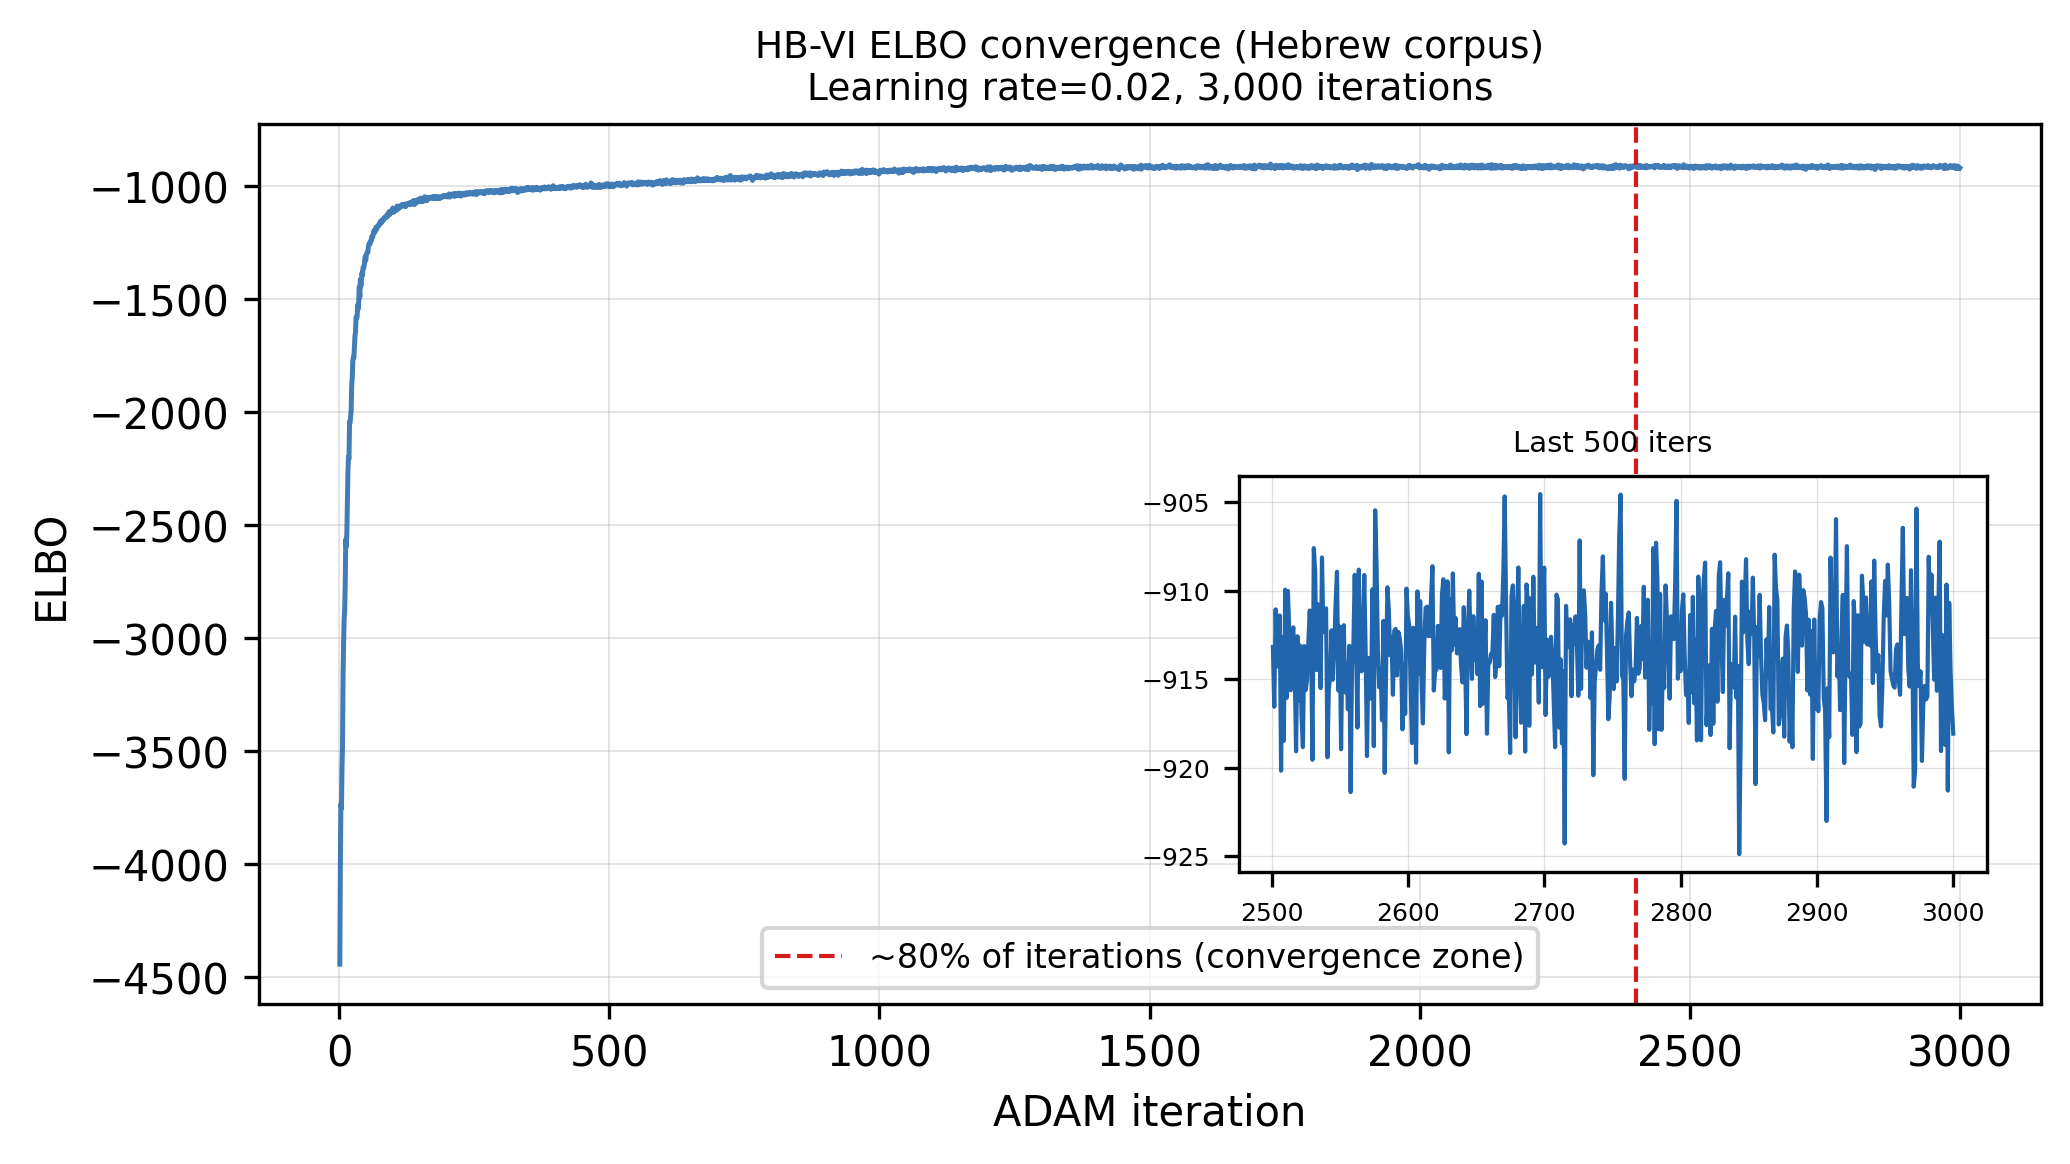
\includegraphics[width=\linewidth]{figures/fig_s9_elbo_convergence.png}
\caption{\textbf{S9 Fig.\ HB-VI ELBO convergence.}
ELBO vs.\ ADAM iteration (learning rate~= 0.02, 3{,}000 iterations).
Dashed line marks the 80\% convergence threshold; inset shows the final
500 iterations confirming near-flat behaviour.}
\label{fig:s9_elbo}
\end{figure}





\begin{figure}[!h]
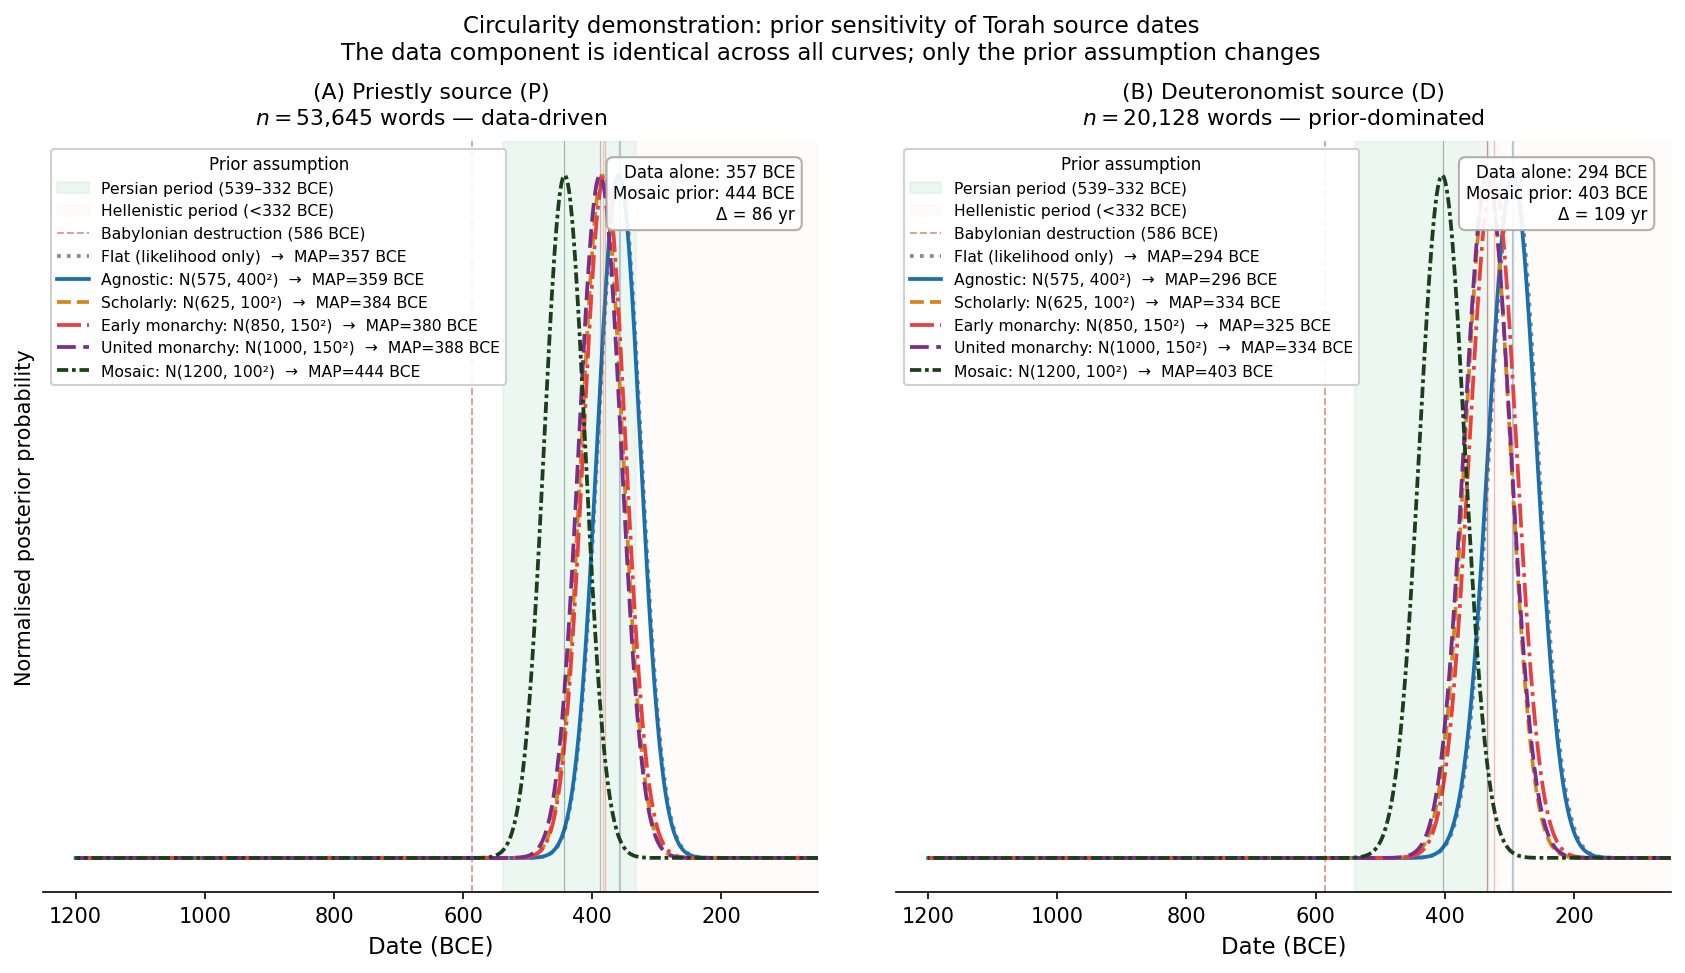
\includegraphics[width=\linewidth]{figures/fig_circularity.png}
\caption{\textbf{S14 Fig.\ Circularity demonstration: prior sensitivity of Torah source dates.}
Normalised MLE-MVN posterior curves for (A) the Priestly source ($n=53{,}645$~words) and
(B) the Deuteronomist source ($n=20{,}128$~words), under six prior assumptions: a data-only
flat prior, the agnostic prior $\mathcal{N}(575,400^2)$, a scholarly prior
$\mathcal{N}(625,100^2)$, an early-monarchy prior $\mathcal{N}(850,150^2)$, a
united-monarchy prior $\mathcal{N}(1000,150^2)$, and a Mosaic-authorship prior
$\mathcal{N}(1200,100^2)$.  The green shading marks the Persian period (539--332~BCE);
the vertical dashed red line marks the Babylonian destruction (586~BCE).  Feature
likelihoods are identical across all curves; only the prior assumption varies.  Even
the Mosaic prior yields MAP dates of 444~BCE (P) and 403~BCE (D), both firmly within
the Persian period.  The pre-exilic Torah date is not recoverable from the
uncontaminated linguistic signal.}
\label{fig:s14_circularity}
\end{figure}

\begin{table}[!ht]
\caption{\textbf{S3 Table.\ Top dating-driving features for the three Documentary Hypothesis source
composites.}
For each source the three features most strongly indicating late and early composition are shown
with their normalized archaism scores (Eq.~\ref{eq:lbh_score}): $s=0$ = CBH-like, $s=1$ =
LBH-like, $s<0$ = more archaic than the SBH anchor, $s>1$ = more LBH-like than the LBH
anchor.  ``Genre flag'' marks features whose value in this source is plausibly driven by prose
genre rather than date (see text).  All features are computed directly from BHSA morphological
tags and can be verified without running the model.  Each source heading reports both model
estimates: MAP$_{\text{MVN}}$ is the \mvn{} posterior mode under the agnostic prior (the
quantity plotted in Fig.~\ref{fig:timeline}), and MAP$_{\text{HB-VI}}$ is the
corresponding \hbvi{} estimate.  The two models differ by 40--100~yr for these composites
because \hbvi{} pools information across register groups and propagates coefficient
uncertainty, which pulls prior-dominated sources toward their group mean; both models place
all three sources in the Persian-to-Hellenistic period.}
\label{tab:s3_features}
\setlength{\tabcolsep}{4pt}
\begin{tabular}{llp{4.9cm}rp{5.1cm}}
\hline
\textbf{Source} & \textbf{Direction} & \textbf{Feature} & \textbf{Score} & \textbf{Note} \\
\hline
\multicolumn{5}{p{15cm}}{\textit{D source composite (Deuteronomist; MAP$_{\text{MVN}}$ = 292~BCE, MAP$_{\text{HB-VI}}$ = 394~BCE; prior-dominated Class~P, $|\Delta_{AB}|=178$~yr)}} \\
D & Late & \textit{asher} relative particle rate & $+3.31$ & Genre flag: high rate reflects legal-prose relative-clause density, not late date \\
D & Late & \textit{eleh} ``these'' rate         & $+1.26$ & Consistent LBH lexical marker \\
D & Late & Infinitive-construct fraction             & $+1.25$ & LBH syntactic feature \\
D & Early & \textit{anoki} vs.\ \textit{ani} 1sg pronoun & $-1.20$ & Classic SBH marker; archaic divine-speech convention in legal texts \\
D & Early & \textit{sham} ``there'' rate          & $-1.27$ & Classic SBH marker \\
D & Early & \textit{lema'an} ``in order that'' rate & $-1.97$ & Classic SBH marker \\
\hline
\multicolumn{5}{p{15cm}}{\textit{P source composite (Priestly; MAP$_{\text{MVN}}$ = 361~BCE, MAP$_{\text{HB-VI}}$ = 404~BCE; data-driven Class~D, $|\Delta_{AB}|=4$~yr)}} \\
P & Late & Niphal stem rate                          & $+1.39$ & Consistent LBH morphological marker \\
P & Late & Abstract nominal rate                     & $+1.32$ & Consistent LBH feature (high nominal density) \\
P & Late & \textit{eleh} ``these'' rate           & $+1.28$ & Consistent LBH lexical marker \\
P & Early & Infinitive-construct rate                & $+0.15$ & Low inf.\ construct (legal/priestly prose pattern) \\
P & Early & \textit{she-} relative particle rate    & $-0.06$ & Classic SBH marker; no late relative pronoun \\
P & Early & Construct-state noun count               & $-0.04$ & High construct ratio (SBH nominal style) \\
\hline
\multicolumn{5}{p{15cm}}{\textit{JE source composite (Jahwist-Elohist; MAP$_{\text{MVN}}$ = 435~BCE, MAP$_{\text{HB-VI}}$ = 531~BCE; prior-dominated Class~P, $|\Delta_{AB}|=172$~yr)}} \\
JE & Late & Wayyiqtol fraction of narrative verbs    & $+1.51$ & Genre flag: high rate reflects narrative genre, not exclusively date \\
JE & Late & \textit{bet} preposition rate          & $+1.42$ & Consistent LBH prose marker \\
JE & Late & \textit{waw} conjunction rate          & $+1.28$ & Consistent LBH narrative marker \\
JE & Early & \textit{she-} relative particle rate   & $-0.05$ & Classic SBH marker; no late relative pronoun \\
JE & Early & \textit{anoki} vs.\ \textit{ani} 1sg pronoun & $-0.46$ & SBH marker \\
JE & Early & \textit{sham} ``there'' rate          & $-0.56$ & Classic SBH marker \\
\hline
\multicolumn{5}{p{15cm}}{\small Scores are computed as $s_j = (x_j - \hat{f}_j(720\,\text{BCE})) /
(\hat{f}_j(250\,\text{BCE}) - \hat{f}_j(720\,\text{BCE}))$ where $\hat{f}_j$ is the OLS-fitted
feature trajectory.  Scores $>1$ indicate the feature value exceeds the LBH anchor level.
Features marked ``Genre flag'' should be interpreted with caution because the training corpus
contains no legal-prose texts from the Persian or Hellenistic period; see text.} \\
\end{tabular}
\end{table}

\begin{table}[!ht]
\caption{\textbf{S4 Table.\ Robustness of source MAP dates to exclusion of genre-confounded features.}
MLE-MVN MAP dates for D, P, and JE under progressive feature exclusion.  R1 removes
\textit{asher} frequency (genre-flagged for D; see S3~Table).  R2 additionally removes
wayyiqtol fraction (genre-flagged for JE).  R3 removes all features with normalized archaism
score $|s|>2.5$ for any source.  Feature vectors are reconstructed from normalized archaism
scores (see Methods); absolute dates carry a minor approximation error, so the shift column
$\Delta$ is the primary quantity of interest.  R2 and R3 produce results identical to R1,
confirming that \textit{asher} is the sole high-leverage outlier.  All sources remain in the
Persian-to-Hellenistic period under all exclusion schemes.}
\label{tab:s4_robustness}
\resizebox{\linewidth}{!}{%
\begin{tabular}{lrrrrr}
\hline
\textbf{Source} & \textbf{Baseline (BCE)} & \textbf{R1: drop \textit{asher} (BCE)} & \textbf{$\Delta$ (yr)} & \textbf{R2 = R3 (BCE)} & \textbf{Period} \\
\hline
D (Deuteronomist)     & 313 & 387 & $+74$ & 387 & Persian \\
P (Priestly)          & 347 & 368 & $+21$ & 368 & Persian \\
JE (Jahwist-Elohist)  & 442 & 456 & $+14$ & 456 & Persian/Hellenistic \\
\hline
\multicolumn{6}{p{0.96\linewidth}}{\small Baseline dates use agnostic prior (Mode~B, $\mathcal{N}(575,400^2)$~BCE) to isolate
the data signal from prior assumptions.  Positive $\Delta$ indicates shift toward more
recent date after feature exclusion.  ``Persian period'' = 539--332~BCE; ``Persian/Hellenistic''
= 539--300~BCE.  The 74~yr shift for D after excluding \textit{asher} confirms
that the dominant late signal in D is genre-confounded; the remaining Persian-period date
reflects the contribution of the remaining late lexical markers (\textit{eleh}, infinitive
construct; see S3~Table).} \\
\end{tabular}}%
\end{table}

\begin{table}[!ht]
\caption{\textbf{S5 Table.\ Corpus word counts for training texts and out-of-sample sources.}
All word counts are morphological words (BHSA) excluding coordinating conjunctions.
The 19 training texts span 760--330~BCE and cover prophetic, poetic, narrative, and
wisdom registers; three additional texts (Habakkuk, Haggai, Daniel) serve as
cross-validation holdouts for the HB-VI model.  Documentary Hypothesis source composites
and sub-source divisions are excluded from both training and validation; their dates are
derived solely from the model posterior.  Texts below $\sim$1{,}000~words produce
noticeably wider posteriors due to sampling noise in feature estimates (see Fig.~S10).}
\label{tab:s5_corpus}
\begin{tabular}{lllrr}
\hline
\textbf{Text} & \textbf{Date (BCE)} & \textbf{Genre} & \textbf{Words} & \textbf{Role} \\
\hline
\multicolumn{5}{l}{\textit{(A) Training corpus and cross-validation holdouts (oldest to most recent)}} \\
  Amos                                   & $760\pm15$       & Prophecy     &   2,780 & Training \\
  Hosea                                  & $725\pm20$       & Prophecy     &   3,146 & Training \\
  Micah                                  & $720\pm20$       & Prophecy     &   1,895 & Training \\
  Isaiah (chs.\ 1--39)                   & $700\pm15$       & Prophecy     &  13,504 & Training \\
  Zephaniah                              & $630\pm15$       & Prophecy     &   1,037 & Training \\
  Nahum                                  & $620\pm20$       & Prophecy     &     746 & Training \\
  Habakkuk                               & $605\pm20$       & Prophecy     &     897 & HB-VI holdout \\
  Jeremiah                               & $590\pm15$       & Prophecy     &  14,539 & Training \\
  Lamentations                           & $586\pm20$       & Poetry       &   1,945 & Training \\
  Ezekiel                                & $570\pm15$       & Prophecy     &  26,182 & Training \\
  Deutero-Isaiah (chs.\ 40--55)          & $550\pm20$       & Prophecy     &   5,738 & Training \\
  Haggai                                 & $520\pm5$        & Prophecy     &     877 & HB-VI holdout \\
  Zechariah (chs.\ 1--8)                 & $518\pm5$        & Prophecy     &   2,484 & Training \\
  Trito-Isaiah (chs.\ 56--66)            & $500\pm100$      & Prophecy     &   3,689 & Training \\
  Malachi                                & $460\pm20$       & Prophecy     &   1,187 & Training \\
  Jonah                                  & $400\pm50$       & Narrative    &     985 & Training \\
  Chronicles                             & $350\pm30$       & Narrative    &  35,330 & Training \\
  Esther                                 & $350\pm50$       & Narrative    &   4,621 & Training \\
  Ezra                                   & $350\pm75$       & Narrative    &   5,268 & Training \\
  Nehemiah                               & $350\pm75$       & Narrative    &   7,842 & Training \\
  Ecclesiastes                           & $330\pm80$       & Wisdom       &   4,233 & Training \\
  Daniel                                 & $167\pm10$       & Mixed        &   8,072 & HB-VI holdout \\
\hline
\multicolumn{5}{l}{\textit{(B) Out-of-sample Documentary Hypothesis sources (excluded from all model fitting)}} \\
  D source composite                     & ---              & Legal        &  20,128 & Out-of-sample \\
  P source composite                     & ---              & Legal        &  53,645 & Out-of-sample \\
  JE source composite                    & ---              & Narrative    &  40,867 & Out-of-sample \\
  D Code (Deut 12--26)                   & ---              & Legal        &   7,353 & Out-of-sample \\
  D Frame (Deut 1--11, 27--34)           & ---              & Narrative    &  11,993 & Out-of-sample \\
  D Song (Deut 32--33)                   & ---              & Other        &     782 & Out-of-sample \\
  Lev Holiness Code (17--26)             & ---              & Legal        &   5,958 & Out-of-sample \\
  Lev Priestly (1--16)                   & ---              & Legal        &  10,496 & Out-of-sample \\
\hline
\multicolumn{5}{p{14cm}}{\small HB-VI holdouts (Habakkuk, Haggai, Daniel) are withheld
from \emph{all} model fitting; their MAP dates assess cross-validation accuracy only
(Fig.~9).  The training/holdout distinction applies to HB-VI; all 22 texts in panel~(A)
appear in MLE-MVN training.  D~Song (782~words) should be treated with caution given its
small size and poetic genre.  CBH = Classical Biblical Hebrew;
LBH = Late Biblical Hebrew; Transitional = texts with mixed register features.} \\
\end{tabular}
\end{table}

\begin{table}[!ht]
\caption{\textbf{S6 Table.\ Prior-sweep MAP dates for the three Torah source composites.}
MLE-MVN MAP dates (BCE) for the Priestly (P), Deuteronomist (D), and Yahwist-Elohist (JE)
source composites under six prior scenarios ranging from an uninformative flat (data-only)
prior to a Mosaic-authorship prior $\mathcal{N}(1200,100^2)$.  Feature vectors are held
fixed across all rows (reconstructed from normalized archaism scores; see Methods and
Fig.~S14); only the prior assumption changes.  The Babylonian destruction (586~BCE),
the Cyrus decree (539~BCE), and the onset of the Hellenistic period (332~BCE) are shown
for reference.  None of the six scenarios recovers a pre-exilic MAP date for any source;
the data signal is strong enough to anchor all three sources in the Persian period even
under the most extreme traditional prior.}
\label{tab:s6_prior_sweep}
\begin{tabular}{lccrrrc}
\hline
\textbf{Prior scenario} &
$\boldsymbol{\mu_0}$ (BCE) & $\boldsymbol{\sigma_0}$ (yr) &
\textbf{P MAP} & \textbf{D MAP} & \textbf{JE MAP} & \textbf{Period} \\
\hline
Flat (data only)
  & --- & --- & 357 & 294 & 434 & Persian \\
Agnostic $\mathcal{N}(575,400^2)$
  & 575 & 400 & 359 & 296 & 434 & Persian \\
Scholarly $\mathcal{N}(625,100^2)$
  & 625 & 100 & 384 & 334 & 453 & Persian \\
Early monarchy $\mathcal{N}(850,150^2)$
  & 850 & 150 & 380 & 325 & 453 & Persian \\
United monarchy $\mathcal{N}(1000,150^2)$
  & 1000 & 150 & 388 & 334 & 461 & Persian \\
Mosaic $\mathcal{N}(1200,100^2)$
  & 1200 & 100 & 444 & 403 & 511 & Persian \\
\hline
\multicolumn{7}{p{14.5cm}}{\small Feature vectors reconstructed from normalized
archaism scores (archaism\_by\_feature.csv) via OLS back-transform; see Methods.
Word-count scaling $\mathrm{clip}(n/5000,1,5)$ applied (P $n=53{,}645$;
D $n=20{,}128$; JE $n=40{,}867$ words).  The P--Mosaic shift of 87~yr across
the full prior range confirms the data-driven classification from the prior
sensitivity analysis ($|\Delta_{AB}|=4$~yr; Table~3).} \\
\end{tabular}
\end{table}


\end{document}

\begin{table}[!ht]
\centering
\caption{\textbf{S2 Table.\ Screening power and false-discovery cost at $N=23$.}
For each nominal $\alpha$: features retained from $K=55$ candidates, the number
expected under the null, the estimated false discovery proportion, and the minimum
$|\rho|$ detectable at 80\% power.  Benjamini-Hochberg at $q=0.10$ independently
retains 7 features.  The operating point used throughout is $\alpha=0.05$; the
35-feature specification of earlier versions of this work corresponds to
$\alpha \approx 0.3$, where more than half the retained features are expected to
be noise.}
\begin{tabular}{rrrrr}
\hline
$\mathbf{\alpha}$ & \textbf{retained} & \textbf{expected null} & \textbf{est.\ FDP} & \textbf{min $|\rho|$ @80\%} \\
\hline
0.01 & 6 & 0.6 & 0.10 & 0.68 \\
0.05 & 14 & 2.8 & 0.20 & 0.58 \\
0.10 & 18 & 5.5 & 0.30 & 0.53 \\
0.15 & 25 & 8.2 & 0.33 & 0.49 \\
0.20 & 27 & 10.9 & 0.40 & 0.46 \\
0.25 & 30 & 13.6 & 0.45 & 0.43 \\
0.30 & 30 & 16.3 & 0.54 & 0.41 \\
\hline
\end{tabular}
\label{tab:s2_power}
\end{table}

\begin{table}[!ht]
\centering
\caption{\textbf{S5 Table.\ Token counts for all units.}
Counts are from the BHSA extraction used for every feature rate in this paper.
Source composites overlap the books that contain them and are not independent;
D source and Deuteronomy are the same text.}
\begin{tabular}{lrl}
\hline
\textbf{Unit} & \textbf{Words} & \textbf{Role} \\
\hline
Chronicles & 35{,}330 & training \\
Ezekiel & 26{,}182 & training \\
Jeremiah oracle & 14{,}539 & holdout \\
Isaiah 1--39 & 13{,}504 & training \\
Nehemiah & 7{,}842 & training \\
Isaiah 40--55 & 5{,}738 & training \\
Ezra & 5{,}268 & training \\
Esther & 4{,}621 & training \\
Ecclesiastes & 4{,}233 & training \\
Isaiah 56--66 & 3{,}689 & training \\
Daniel (Heb.) & 3{,}437 & training \\
Hosea & 3{,}146 & training \\
Amos & 2{,}780 & training \\
Zechariah 1--8 & 2{,}484 & training \\
Zechariah 9--14 & 1{,}987 & training \\
Lamentations & 1{,}945 & training \\
Micah & 1{,}895 & training \\
Joel & 1{,}318 & training \\
Malachi & 1{,}187 & training \\
Zephaniah & 1{,}037 & training \\
Jonah & 985 & training \\
Habakkuk & 897 & training \\
Haggai & 877 & holdout \\
Nahum & 746 & training \\
Obadiah & 392 & training \\
\hline
P source & 54{,}435 & target \\
JE source & 37{,}752 & target \\
Genesis & 28{,}764 & target \\
Exodus & 23{,}748 & target \\
Numbers & 23{,}188 & target \\
Genesis JE & 22{,}409 & target \\
Deuteronomy & 20{,}128 & target \\
D source & 20{,}128 & target \\
Leviticus & 17{,}099 & target \\
Jeremiah Dtr & 15{,}197 & target \\
D Frame & 11{,}993 & target \\
Exodus JE & 11{,}780 & target \\
Leviticus P & 10{,}496 & target \\
D Code & 7{,}353 & target \\
Holiness Code & 5{,}958 & target \\
Numbers JE & 3{,}563 & target \\
D Song & 782 & target \\
Song of Deborah & 462 & target \\
Song of the Sea & 433 & target \\
\hline
\end{tabular}
\label{tab:s5_words}
\end{table}
